\chapter{Motivation \& Tools from the Continuum}
\label{chap:background}

In this chapter, we lay out the physics context of this work and some theoretical machinery that was useful in our studies. This section consists of a definition and empirical status of the standard model. Then, we will expand on the details of the specific sector we are interested in - the flavour sector and the CKM matrix.

We will then move onto some lay down some physics machinery used in our work, namely QCD and chiral symmetry, and effective field theories for heavy quarks.

\section{Testing the Standard Model}

The Standard Model of Particle Physics (SM) is, so far, the most successful theory for describing fundamental particles and their interactions. It is an effective Yang-Mills quantum field theory. It is most succinctly defined by listing its symmetries, field content, and the irreducible representations (irreps) of the symmetries that those fields transform under.

The symmetries are the following. The Lorentz group $SO(3,1)$, the group of coordinate transformations that leave the Minkowski metric invariant, which can be decomposed into $SU(2)_l\times SU(2)_r$ ({\it{left-handed}} and {\it{right-handed}}). We denote an irrep as $(a,b)$ where $a$ is the $\sigma^z$ eigenvalue under $SU(2)_l$ transforms, and $b$ is that of $SU(2)_r$. Then there are internal local gauge symmetries:
\begin{align}
  SU(3)_C\times SU(2)_L \times U(1)_Y,
\end{align}
irreps of which we denote with $(x,y,z)$, where $x,y$ are the $SU(3)_C$ and $SU(2)_W$ irreps and $z$ is the charge under $U(1)_Y$.

The field content is: gauge bosons for each generator of the above gauge symmetries, each transforming in the adjoint of their corresponding symmetry and in the $(1/2,1/2)$ irrep of the Lorentz group, denoted $B_{\mu}$, $W_{\mu}$, $G_{\mu}$ respectively. There are 6 $SU(2)_L$ doublets in the $(1/2,0)$ Lorentz irrep;
\begin{align}
  Q_{1,2,3} =&
  \begin{pmatrix} u_L \\ d_L \end{pmatrix},
  \begin{pmatrix} c_L \\ s_L \end{pmatrix},
  \begin{pmatrix} t_L \\ b_L \end{pmatrix}
  \quad,\quad
  (\mathbf{3},\mathbf{2},1/6) \\
  L_{1,2,3} =&
  \begin{pmatrix} \nu_{e,L} \\ e_L \end{pmatrix},
  \begin{pmatrix} \nu_{\mu,L} \\ \mu_L \end{pmatrix},
  \begin{pmatrix} \nu_{\tau,L} \\ \tau_L \end{pmatrix}
  \quad,\quad
  (\mathbf{1},\mathbf{2},-1)
\end{align}
and 9 $SU(2)_L$ singlets in the $(0,1/2)$ Lorentz irrep;
\begin{align}
  u^R_{1,2,3} &= u_R, c_R, t_R\quad,\quad (\bar{\mathbf{3}},\mathbf{1},2/3) \\
  d^R_{1,2,3} &= d_R, s_R, b_R\quad,\quad (\bar{\mathbf{3}},\mathbf{1},-1/3) \\
  e^R_{1,2,3} &= e_R, \mu_R, \tau_R\quad,\quad (\mathbf{1},\mathbf{1},-1).
\end{align}
We have also listed the SM gauge irreps next to each definition. There is also in principle a further set of right-handed $SU(2)_L$ singlets, $\nu^R_{1,2,3} = (\nu_{e,R}, \nu_{\mu,R}, \nu_{\tau,R})$, but these are singlets of the entire SM gauge group so in a phenomenological sense very much 'not there'. There is also a Lorentz scalar $SU(2)_L$ doublet, the Higgs $H$, with in gauge irrep $({\bf{1}},{\bf{2}},1/2)$ that obtains a vacuum expectation value under $\sim 200$GeV and causes a breaking of the above gauge group to $SU(3)_C\times U(1)_E$, where $U(1)_E$ is the electroweak gauge group mediated by the photon.
\\ \\
There is at present no confirmed evidence of physics beyond the SM (or {\it{new physics}} (NP)), besides the presence of neutrino ($\nu$) masses. However, there are a number of problems with the SM that heavily imply that there must be new physics. Among the most famous sources of concern are:
\begin{itemize}
\item
  {\bf{Dark Matter \& Dark Energy}} - an estimated 96\% of the content of the universe is dark matter and dark energy, that does not interact with the SM gauge group (only via gravity), so cannot be explained by the SM.
\item
  {\bf{Matter/Antimatter Asymmetry}} - the SM requires there to be an equal amount of matter and antimatter in the universe, however, we observe a massive dominance of matter over antimatter.
\item
  {\bf{Neutrino Oscillations}} - different species of neutrinos oscillate into each other over time, there is no SM mechanism to explain this.
\item
  {\bf{The Hierarchy Problem}} - the SM is 'finely tuned', the chances of the Higgs choosing its current vacuum expectation value is estimated to be one in $\sim 10^{45}$.
\end{itemize}

The central goal of particle physics is currently to pin down evidence against the standard model. Only once we have detailed knowledge of how it breaks down will theorists be able to uniquely determine a new theory of fundamental physics.

There are many promising approaches to achieve this. They are traditionally separated into
\begin{itemize}
\item
  {\bf{The Energy Frontier}} - explore the highest possible energies reachable with accelerators, directly looking for new physics via the production and identification of new states of matter.
\item
  {\bf{The Cosmic Frontier}} - use the universe as an experimental laboratory and observatory,  taking advantage of naturally occurring events to observe indications of new interactions.
\item
  {\bf{The Intensity Frontier}} - use intense sources of particles from accelerators, reactors, the sun and the atmosphere to make ultra-precise measurements and find subtle deviations from SM predictions.
\end{itemize}
The work in this thesis contributes to the third approach. There is a rising tide of more and more SM observables being measured and predicted more and more precisely. It is only a matter of time until one of these observables yields a statistically significant deviation from the SM.

\section{Flavour-Changing Charged Currents}
\label{sec:fccc}

The SM tests relevant to this work are on quark flavour-changing interactions. Here we will detail the parts of the SM relevant to these interactions.

The $SU(2)_L$ gauge symmetry of the SM is mediated by the vector boson $W=W^1\tau_1 + W^2\tau_2 + W^3\tau_3$, where $\tau_i$ are the three $SU(2)$ generators acting on the $SU(2)_L$ doublets defined in the last section. It is convenient to redefine the fields $W = W^+ ( \tau_0 + i\tau_1 ) + W^- ( \tau_0 - i\tau_1 ) + W^3 \tau_3$.\, $W^{\pm},W^3$ are the stationary states at low energies due to electroweak symmetry breaking.

The part of the SM Lagrangian that describes the coupling of $W^{\pm}$ to fermions is given by
\begin{align}
  \mathcal{L}_{\text{FCCC}} = {e\over \sqrt{2}\sin\theta_W} \left( \bar{u}_L^i \slashed{W}^+ d_L^i + \bar{d}_L^i \slashed{W}^- u_L^i + \bar{\nu}_L^i \bar{W}^+ e_L^i + \bar{e}_L^i \slashed{W}^- \nu_L^i \right),
  \label{eq:FCCC}
\end{align}
where $e$ is the electron charge, $\theta_W$ is the Weinberg angle (a parameter of the SM), and $\slashed{V} = \gamma^{\mu} V_{\mu}$ where $\gamma^{\mu}$ are members of the Clifford algebra acting on fermion spin components. To understand the interactions these terms cause we must also consider the mass terms for the fermions:
\begin{align}
  \mathcal{L}_{\text{mass}} = y_{ij}^u \left({v\over \sqrt{2}}\right) u_L^i u_R^j + y_{ij}^d \left({v\over \sqrt{2}}\right) d_L^i d_R^j + y_{ij}^e \left({v\over \sqrt{2}}\right) e_L^i e_R^j.
\end{align}
These terms come from the coupling of the fermions to the Higgs field, where the Higgs has taken a vacuum expectation value $v$ at low energies. $y^{u,d,e}_{ij}$ are the Yukawa matrices, parameterising the coupling of the fermions to the Higgs, consisting of free SM parameters. The absence of right-handed neutrinos forbids an analagous term for neutrinos.

Due to these nondiagonal mass terms, the fundamental fermion fields are not stationary states. To obtain a more useful representation, one rotates the fields to diagonalise these terms
\begin{align}
  \psi^L_i\to L^{\psi}_{ij} \psi^L_j \,,\, \psi_R^i \to R^{\psi}_{ij} \psi_R^j,
\end{align}
where $\psi=u,d$ or $e$, and we fix $L^{\psi}_{ij}$,$R^{\psi}_{ij}$ according to
\begin{align}
  y^{\psi} \left({v\over \sqrt{2}}\right)= L^{\psi} M^{\psi} R^{\psi}
\end{align}
where $M^{\psi}$ is diagonal. This results in diagonal mass terms, but also has an effect on $\mathcal{L}_{\text{FCCC}}$:
\begin{align}
  \mathcal{L}_{\text{FCCC}} = {e\over \sqrt{2}\sin\theta_W} \left( V_{ij} \bar{u}_L^i \slashed{W}^+  d_L^j + V_{ij}^* \bar{d}_L^i \slashed{W}^- u_L^j + \bar{\nu}_L^i \slashed{W}^+ e_L^i + \bar{e}_L^i \slashed{W}^- \nu_L^i \right).
  \label{eq:FCCC}
\end{align}
$V = L^{u\,\dagger} L^d$ is by construction a unitary matrix ($V^{\dagger}V = (L^{d\,\dagger} L^u)(L^{u\,\dagger} L^d) = L^d L^{d\,\dagger} = 1)$. $V$ is the famous Cabibbo–Kobayashi–Maskawa (CKM) matrix, consisting of parameters that must be fixed by experiment.

There is no non-diagonal flavour structure in the last two terms because we have redefined the neutrino fields: $\nu_L \to L^{e\,\dagger} \nu_L$, absorbing the rotation of the $e_L$ fields. This can be done with impunity due to the lack of neutrino mass terms. While the SM does not include neutrino mass terms, it has in fact been experimentally confirmed that neutrinos have mass. It is however known that these masses are extremely small in comparison to the scales of the SM ($m_{\nu}\lessapprox 0.05$eV). Any lepton flavour-changing effect this could in principle have would be much smaller than the current sensitivity of any experiment, for example, $\mathcal{B}(\mu\to \tau \gamma) \simeq 10^{-34}$.

Another useful redefinition is to collect the left-handed and right-handed fermion fields into Dirac spinors $\psi$:
\begin{align}
  \psi = \psi_L + \psi_R \,\,,\,\, \psi_L = {1\over 2}\left(1-\gamma^5 \right) \psi \,\,,\,\, \psi_R = {1\over 2}\left(1+\gamma^5\right) \psi
\end{align}
In terms of Dirac spinors, $\mathcal{L}_{\text{FCCC}}$ can be written as
\begin{align}
  \mathcal{L}_{\text{FCCC}} =& {e \over \sqrt{2} \sin \theta_W} \left( V_{ij} J^{ij}_{\mu} W^{+\,\mu} + V^*_{ij} J^{ij\,\dagger}_{\mu} W^{-\,\mu} +
  L^{ii}_{\mu} W^{+\,\mu} + L^{ii\,\dagger}_{\mu} W^{-\,\mu}
  \right), \\
  &L^{ij}_{\mu} = {1\over2}\left(\bar{\nu}^i \gamma_{\mu} e^j - \bar{\nu}^i \gamma_5 \gamma_{\mu} e^j\right), \\
  &J^{ij}_{\mu} = {1\over2}\left(\bar{u}^i \gamma_{\mu} d^j - \bar{u}^i \gamma_5 \gamma_{\mu} d^j\right) \equiv V^{ij}_{\mu} - A^{ij}_{\mu}.
\end{align}
$J^{ij}_{\mu}$ is known as the Flavour-Changing Charged Current (FCCC). It is often broken up into the {\it{vector}} and {\it{axial-vector}} components, $V_{\mu}$ and $A_{\mu}$ respectively, since these two componets can be categorised according to their transformations under the Lorentz group. $V_{\mu}$ is labelled $1^+$, where the $1$ represents it's total spin, and the $+$ represents it's positive parity $P: V_{\mu} \to V_{\mu}$. $A_{\mu}$ is instead labelled $1^-$, due to it's negative parity $P: A_{\mu} \to - A_{\mu}$.

We can now turn to the physical consequences of $\mathcal{L}_{\text{FCCC}}$. The interactions given in this part of the Lagrangian describe a quark changing flavour while emitting a $W^{\pm}$ boson. The propensity for flavour $i$ to decay into another flavour $j$ is governed in part by energy constraints and in part by the associated CKM element $V_{ij}$. These
interactions at the quark level mediate meson decays, namely leptonic and semileptonic decays, described in section \ref{sec:weakdecays}.

The deviation of $V_{ij}$ from a unit matrix breaks some of the symmetries of the SM. $\mathcal{L}_{\text{SM}}-\mathcal{L}_{\text{FCCC}}$ has the property that one can independently rephase each of the quark fields, $q_i\to e^{i\theta_i}q_i$, a global $U(1)$ symmetry for each quark flavour. This implies, via Noether's theorem, that the number of quarks of each flavour, $N_i$, is conserved. However, $\mathcal{L}_{\text{FCCC}}$ breaks this symmetry $U(1)^6\to U(1)$, where there is only a remnant symmetry of transforming all flavours by the same phase. Individual quark flavour number is no longer conserved, but overall quark number is.

Since there is no off-diagonal flavour structure for the Leptons, the equivalent global $U(1)^6$ symmetry for the leptons survives in the SM, and individual lepton flavour number is conserved. This property of the SM is referred to as lepton flavour universality.

\begin{figure}
  \begin{center}
    \vspace{-10pt}
    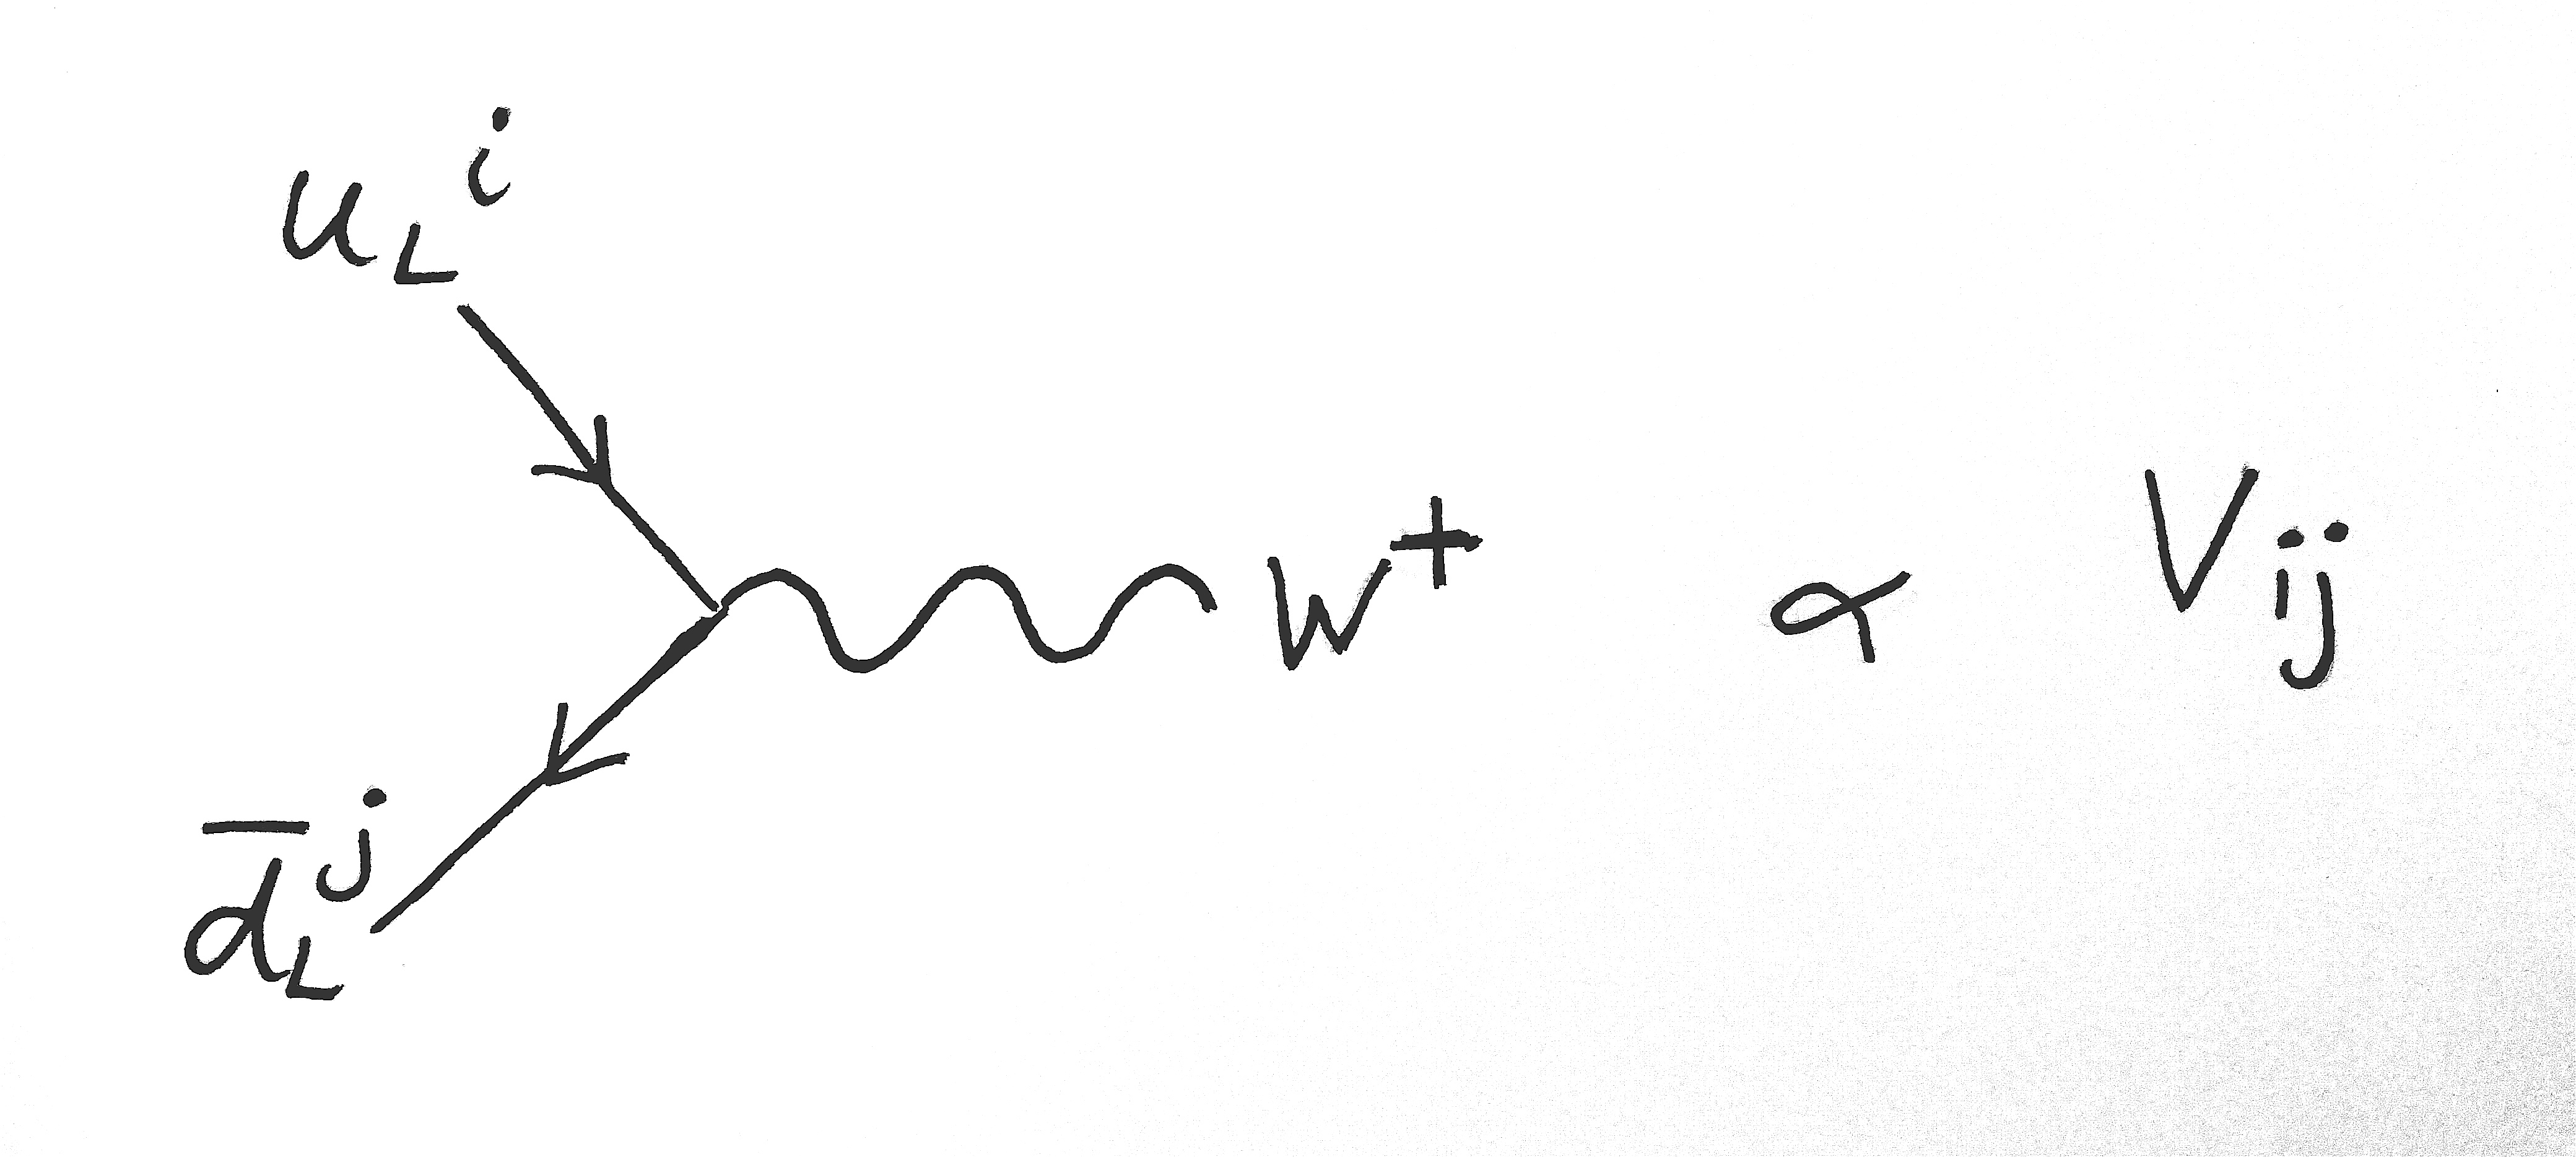
\includegraphics[width=0.5\textwidth]{images/fccc.jpg}
    \vspace{-10pt}
  \end{center}
  \caption{The flavour-changing charged current vertex.}
  \label{fig:fccc}
\end{figure}

\subsection{The CKM Matrix}

The exact values of the CKM matrix elements are of interest in the search for new physics. The CKM matrix is unitary by construction, however, if we were to discover that the values we measure experimentally do not combine to produce a unitary matrix, this would be evidence that the elements we are measuring, in fact, compose a submatrix of a unitary matrix larger than $3\times 3$. This would imply the presence of further, heavier quark generations.

%% Another source of interest in the CKM values is CP violation. CP violation is a global symmetry exhibited by $\mathcal{L}_{\text{SM}}-\mathcal{L}_{\text{FCCC}}$, and physically corresponds to a symmetry between particles and antiparticles. CP violation is one of the famous {\it{Sakarov conditions}}, the conditions necessary for a theory to explain the matter/antimatter asymmetry observed in the universe. CP is generically violated when a parameter of the theory has an imaginary component. The CKM matrix contains one physical phase, making $\mathcal{L}_{\text{FCCC}}$ a source of CP violation. However, the extent of CP violation in the flavour sector is not sufficient to explain the matter/antimatter asymmetry, so the necessary CP violating processes will likely come from new physics beyond the standard model.


%% To understand the structure of the CKM, we must first ask how many independent physical parameters there are. If one imagines that $V$ is purely real, then it becomes an $SO(3)$ matrix, which can be parameterised by 3 angles, so there are $N_{\text{real}} = 3$ independent real parameters. A member of $SU(3)$ has 9 independent parameters, so there must be $N_{\text{im}}=N-N_{\text{real}} = 6$ independent phases.

%% However, we have the freedom to remove some of those phases via a redefinition of the quark fields. $\mathcal{L}_{\text{SM}} - \mathcal{L}_{\text{FCCC}}$ has a global $U(1)^6$ symmetry, a rephasing of each of the 6 quark flavours. One can rephase each flavour without modifying $\mathcal{L}_{\text{SM}} - \mathcal{L}_{\text{FCCC}}$, but with the effect of changing $V$:
%% \begin{align}
%%   V \,\,\to \,\,
%%   \begin{pmatrix}
%%     e^{-ia} & 0 & 0 \\
%%     0 & e^{-ib} & 0 \\
%%     0 & 0 & e^{-ic} \\
%%   \end{pmatrix}
%%   V
%%   \begin{pmatrix}
%%     e^{id} & 0 & 0 \\
%%     0 & e^{ie} & 0 \\
%%     0 & 0 & e^{if} \\
%%   \end{pmatrix},
%% \end{align}
%% where $a,b,c,d,e,f\in \mathbb{R}$. So perhaps one can tune each of these 6 phases to remove all 6 phases in $V$. This is not quite right, we in fact only have the ability to remove 5 of the 6 phases. To see why we can redefine the phases in the following way;
%% \begin{align}
%%   V \,\,\to \,\,
%%   \begin{pmatrix}
%%     e^{-ia} & 0 & 0 \\
%%     0 & e^{-i(a+\alpha)} & 0 \\
%%     0 & 0 & e^{-i(a+\beta)} \\
%%   \end{pmatrix}
%%   V
%%   \begin{pmatrix}
%%     e^{i(a+\gamma)} & 0 & 0 \\
%%     0 & e^{i(a+\delta)} & 0 \\
%%     0 & 0 & e^{i(a+\epsilon)} \\
%%   \end{pmatrix},
%% \end{align}
%% with $\alpha,\beta,\gamma,\delta,\epsilon\in\mathbb{R}$. $a$ is a useless phase - it will always cancel with itself so cannot be used to remove a phase from $V$. Hence, one can remove 5 of the 6 phases by redefining the quark fields, leaving one physical phase in the CKM matrix.

%% This is can be seen as due to the explicit symmetry breaking property of $\mathcal{L}_{\text{FCCC}}$. The inclusion of $\mathcal{L}_{\text{FCCC}}$ breaks the global $U(1)^6$  symmetry down, $U(1)^6 \to U(1)$, where the broken symmetry is a rephasing of all of the quark flavours by the same amount. This says we can modify $\mathcal{L}_{\text{FCCC}}$ by $N_{\text{broken}} = 5$ independent phases without modifying the rest of the Lagrangian.

The CKM contains 3 real parameters and 1 complex phase. There is only one complex phase since we can freely redefine the phases of the quark fields in order to absorb the majority of the phases in the CKM. A common parameterisation is
\begin{align}
  V =
  \begin{pmatrix}
    1 & 0 & 0 \\
    0 & \cos\theta_{23} & \sin\theta_{23} \\
    0 & -\sin\theta_{23} & \cos\theta_{23} \\
  \end{pmatrix}
  \begin{pmatrix}
    1 & 0 & \sin\theta_{12}e^{i\delta} \\
    0 & 1 & 0  \\
    -\sin\theta_{13} e^{i\delta} & 0 & \cos\theta_{13} \\
  \end{pmatrix}
  \begin{pmatrix}
    \cos\theta_{12} & \sin\theta_{12} & 0  \\
    -\sin\theta_{12} & \cos\theta_{12} & 0 \\
    0 & 0 & 1 \\
  \end{pmatrix}.
\end{align}
A useful parameterisation for understanding the relative sizes of the CKM elements is due to Wolfenstein. Define the Wolfenstein parameter $\lambda = \sin\theta_{12}$, which is known experimentally to be around $\lambda\simeq 0.22$. Then $\cos\theta_{12} = \sqrt{1-\sin^2\theta_{12}} = \sqrt{1-\theta^2} \simeq 1 - \lambda^2/2$. Observing then that $\sin\theta_{23} \sim 0.04 \simeq \lambda^2$ and $\sin\theta_{13} \sim 0.004 \simeq \lambda^3/3$, we can write the matrix as
\begin{align}
  V \simeq
  \begin{pmatrix}
    1 - {1\over 2}\lambda^2 & \lambda & {1\over 3} \lambda^3 e^{i\delta}  \\
    - \lambda & 1 - {1\over 2}\lambda^2 & \lambda^2 \\
    \lambda^3(1-{1\over3} e^{i\delta}) & -\lambda^2 & 1 \\
  \end{pmatrix}
  =
  \begin{pmatrix}
    \order{1} & \order{\lambda} & \order{\lambda^3}  \\
    \order{\lambda} & \order{1} & \order{\lambda^2} \\
    \order{\lambda^3} & \order{\lambda^2} & \order{1} \\
  \end{pmatrix}
\end{align}
There is a clear hierarchy between the values - the CKM matrix is close to the unit matrix. Inter-generational mixing is dominant, dropping from second to first generation is suppressed by $\lambda$, dropping from third to second by $\lambda^2$, and dropping from third to first by $\lambda^3$. The SM supplies no compelling explaination of why this hierarchy exists, it is expected that new physics beyond the SM will supply some natural explaination.

The assumption of unitarity in $V$,
\begin{align}
  V_{ji}^*V_{jk}=\delta_{ik},
  \label{eq:CKMunitarity}
\end{align}
imposes 9 constraints on the CKM elements. Each of these constraints gives a test of the SM, if one of these constraints is found to be violated, this represents evidence of new phyisics. The most studied constraint is given by taking $i=3,k=1$;
\begin{align}
  {V_{ud}V_{ub}^*\over V_{cd} V_{cb}^*} + {V_{td}V_{tb}^* \over V_{cd}V_{cb}^*} + 1 = 0.
\end{align}
This can be visualized as a triangle (known as the {\it{unitarity triangle}}) on the complex plane, as shown in figure \ref{fig:unitaritytriangle_sketch}.

\begin{figure}
  \vspace{-10pt}
  \begin{center}
    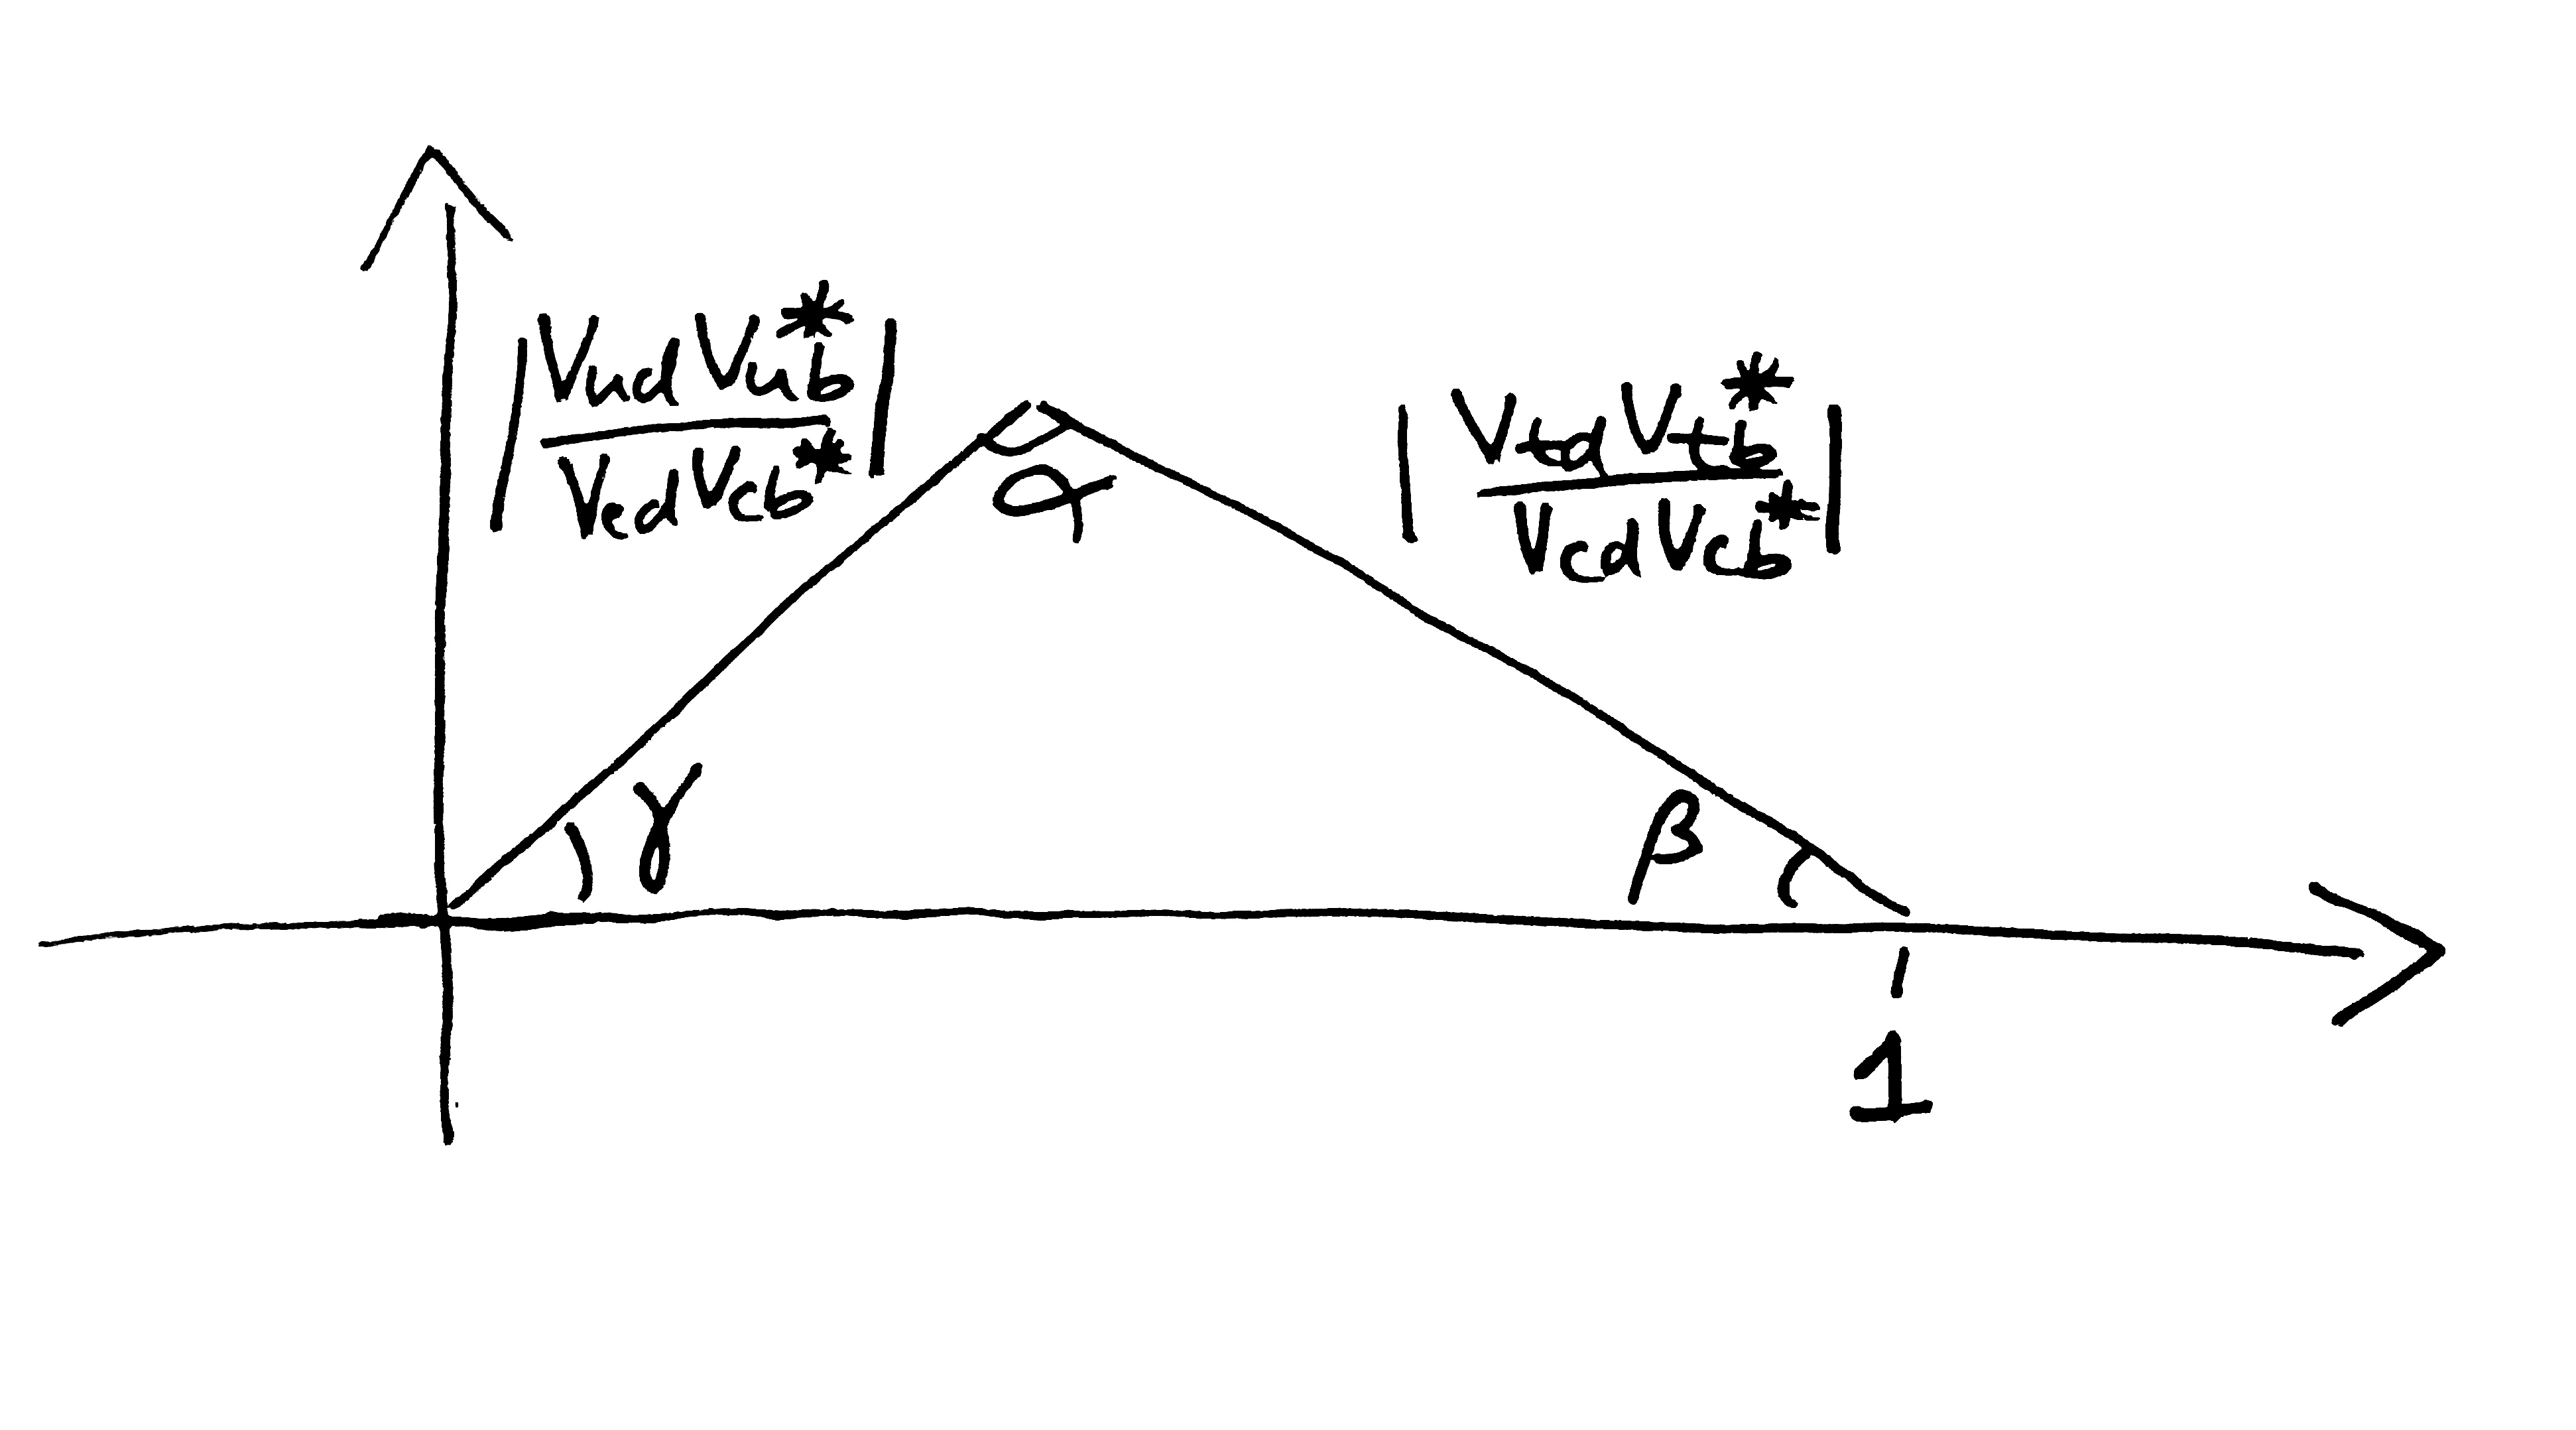
\includegraphics[width=0.7\textwidth]{images/unitaritytriangle_sketch.jpg}
  \end{center}
  \vspace{-40pt}
  \caption{A sketch of the unitarity triangle.}
  \label{fig:unitaritytriangle_sketch}
\end{figure}

For unitarity, the triangle must close, in other words, $\alpha+\beta+\gamma = \pi/2$. Hence to test the CKM unitarity experimentalists measure these angles
\begin{align}
  \alpha = \arg \left( -{V_{td}V_{tb}^*\over V_{ud}V_{ub}^*}\right) \,,\,
  \beta = \arg \left( -{V_{cd}V_{cb}^*\over V_{td}V_{tb}^*} \right) \,,\,
  \gamma = \arg \left( -{V_{ud}V_{ub}^*\over V_{cd}V_{cb}^*} \right).
\end{align}
The unitarity triangle also contains information about CP-violation from flavour-changing charged currents. The so-called Jarlskog invariant, $J=\sin\theta_{12}\sin\theta_{23}\sin\theta_{31}\cos\theta_{12}\cos\theta_{23}\cos\theta_{31}^2\sin\delta$, a measure of CP-violation, is proportional to the area enclosed by the triangle.

The most recent PDG update \cite{PhysRevD.98.030001} reports the following averages for the measurements of CKM elements;
\begin{align}
  |V| = \begin{pmatrix}
    0.97446\pm 0.00010 & 0.22452\pm 0.00044 & 0.00365\pm 0.00012 \\
    0.22438\pm 0.00044 & 0.97359\substack{+0.00010\\-0.00011} & 0.04214\pm 0.00076 \\
    0.00896\substack{+0.00024\\-0.00023} & 0.04133\pm 0.00074 & 0.999105\pm 0.000032 \\
  \end{pmatrix}.
\end{align}
The averages given here are consistent with unitarity in all avaliable tests. %For example, taking \eqref{eq:CKMunitarity} with $i=k=1$, we find $|V_{ud}|^2+|V_{us}|^2+|V_{ub}|^2 = 0.9994\pm 0.0005$.
The angles of the unitarity triangle currently satisfy $\alpha+\beta+\gamma = (180\pm 7)\degree$. Increasing the precision of CKM determinations are necessary to provide more stringent tests of CKM unitarity.

\begin{figure}
  \vspace{-10pt}
  \begin{center}
    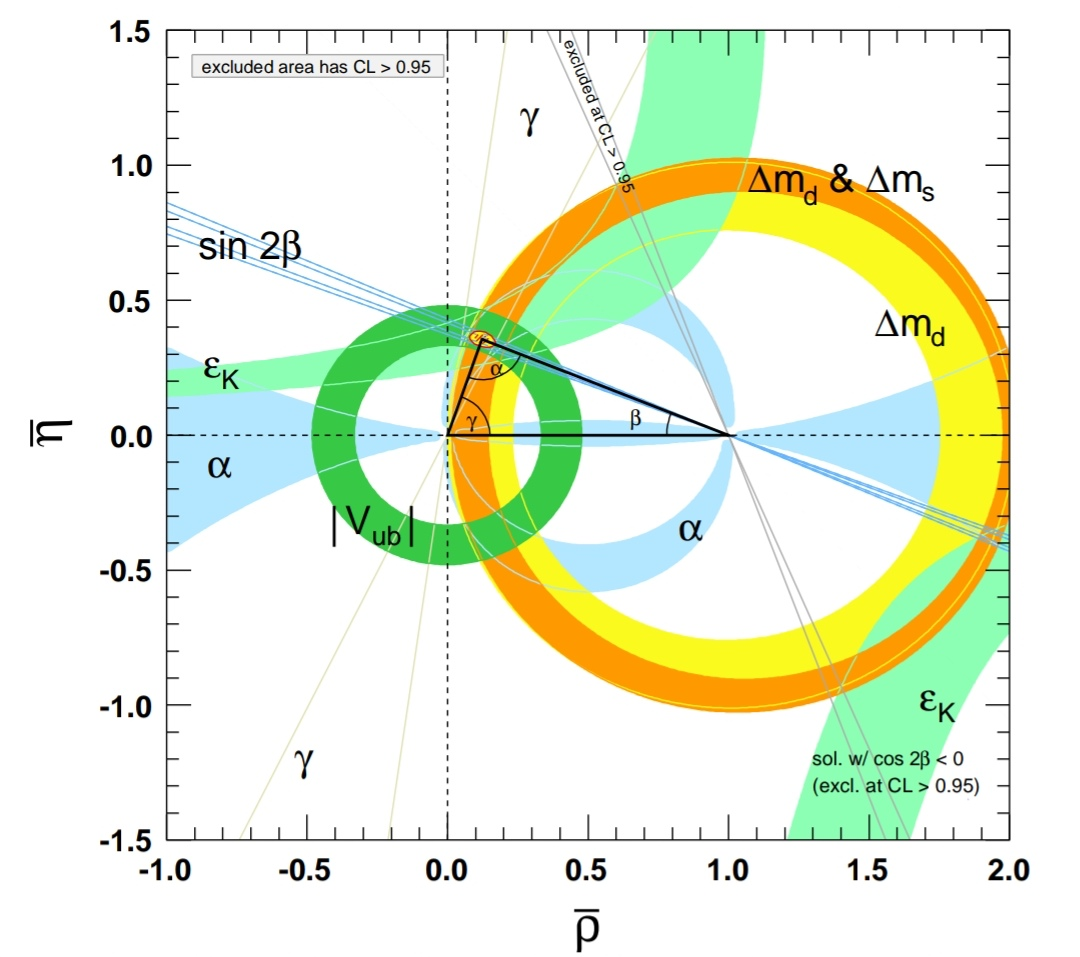
\includegraphics[width=0.6\textwidth]{images/ckmpdg.jpg}
  \end{center}
  \vspace{-25pt}
  \caption{Exclusion regions for the vertices of the CKM triangle from various measurements, coutresy of the most recent PDG update \cite{PhysRevD.98.030001}.}
  \label{fig:ckmpdg}
\end{figure}

\subsection{Weak Decays}
\label{sec:weakdecays}

We now move on to the methods of determining CKM elements. At the confinement scale ($\sim$1GeV and below), quarks are confined by QCD in hardons. At these energies, the dynamics of quarks are only experimentally accessible by probing the dynamics of hadrons. CKM matrix elements are determined by studying hadron decays.

First a word on hadrons. Hadrons are broadly categorized into mesons (charged with one valence quark and one valence antiquark) and baryons (three valence quarks). The entirety of this thesis is concerned with mesons. Mesons are categorized in terms of the flavours they are charged under and their representations under the Lorentz group. We use the same notation as for the quantum numbers of the weak currents; $L^{\pm}$ where $L$ denotes spin and $\pm$ denotes parity. In this thesis, we are concerned mostly with pseudoscalar ($0^-$) and vector ($1^-$) mesons.

Weak decays of mesons are categorized according to the final products:
\begin{itemize}
\item
  {\bf{Leptonic}}: $meson \to leptons$.
\item
  {\bf{Semileptonic}}: $meson \to meson + leptons$.
\item
  {\bf{Hadronic}}: $meson \to mesons$.
\item
  {\bf{Oscillation}}: $meson \to meson$.
\end{itemize}

All of these types of decay are dependent on CKM elements so can in principle to be used for studying them. We are most interested in the first two, leptonic and semileptonic, so will give detail of such decays here.

\begin{figure}
  \vspace{-10pt}
  \begin{center}
    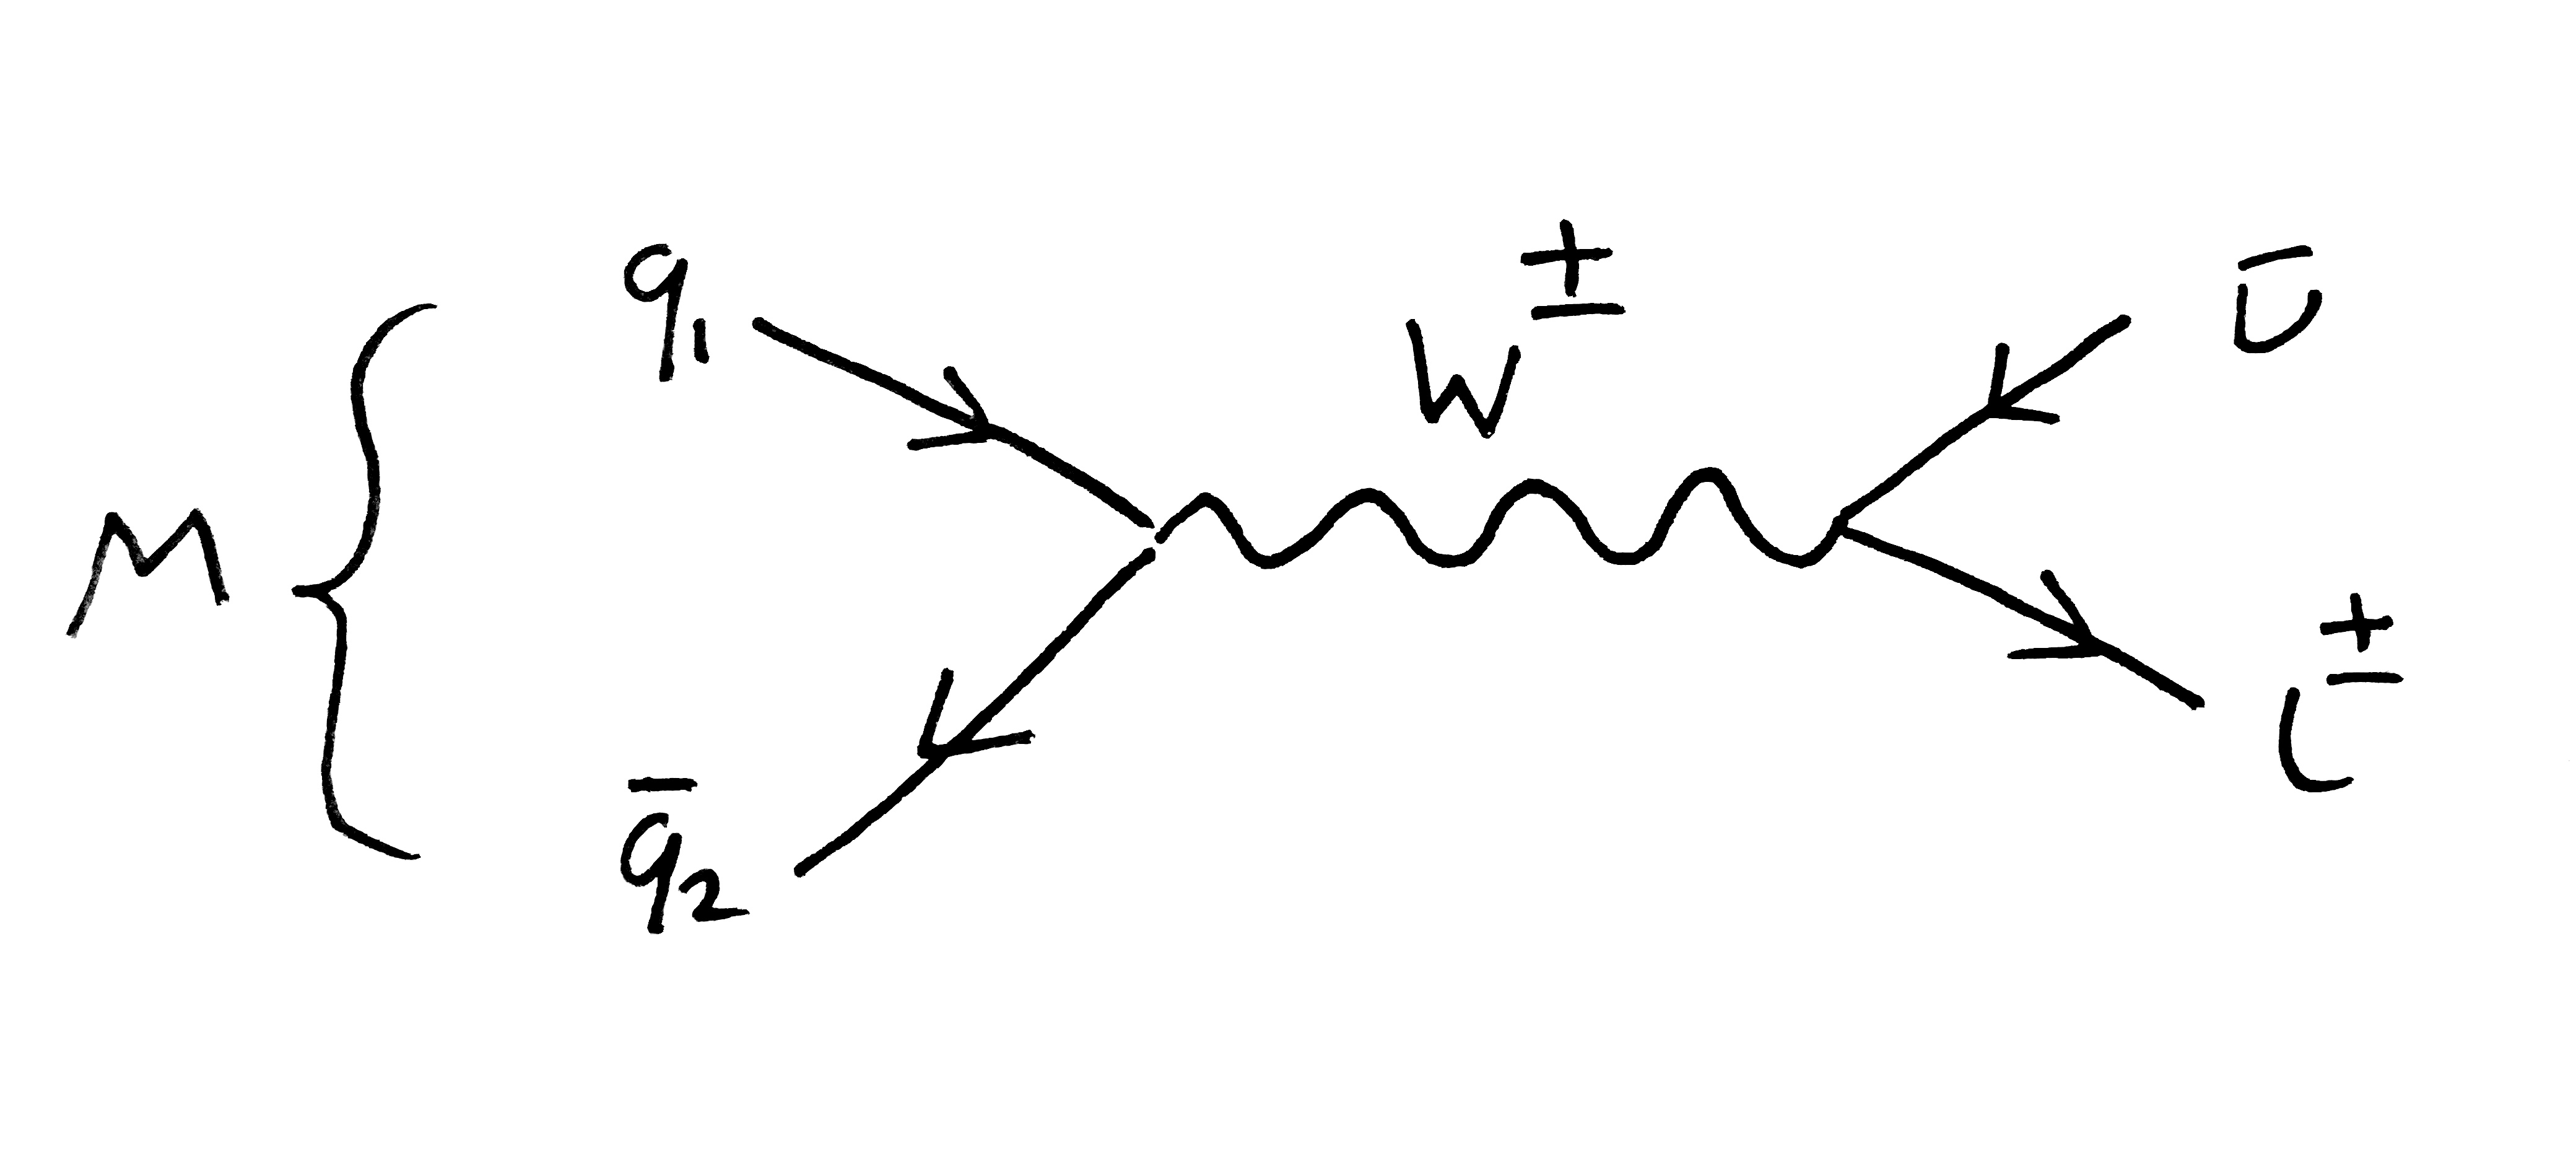
\includegraphics[width=0.6\textwidth]{images/leptonicdecay.jpg}
  \end{center}
  \vspace{-20pt}
  \caption{Leptonic decay of meson $M$ at tree level in the electroweak coupling.}
  \label{fig:leptonicdecay}
\end{figure}

Fig. \ref{fig:leptonicdecay} shows a generic leptonic decay at tree level (in electroweak coupling, virtual quark and gluon lines are implicit). The corresponding amplitude is given by
\begin{align}
  \mathcal{M} = \left({ie\over \sqrt{2}\sin\theta_W}\right) V_{q_1q_2} \langle l\bar{\nu} | L^l_{\mu} D_W^{\mu\nu} J_{\nu}^{q_1q_2} | M \rangle,
\end{align}
where $D_{W}$ is a free $W^{+-}$ propagator, $|M\rangle$ is the ground state of the meson $M$, and $|l\bar{\nu}\rangle$ is a lepton-antineutrino state. We are using the notation $L^l_{\mu}=L^{kk}_{\mu}$, where $l$ indexes the $k$th charged lepton. If the momentum of the meson, $p^2$, is much smaller than the $W$ mass squared, one can integrate out the dynamics of the $W$ to move into the Fermi effective theory \cite{Borasoy:2007yi};
\begin{align}
  \nonumber
  \left({ie\over\sqrt{2}\sin\theta_W}\right)^2 D^{\mu\nu}_W(p^2) &= \left({ie\over\sqrt{2}\sin\theta_W}\right)^2 \left( -ig^{\mu\nu} \over p^2 - M_W^2 \right)
  \\ & = \underbrace{ {i\over M_W^2} \left( ie \over \sqrt{2}\sin\theta_W \right)^2  }_{\equiv -2\sqrt{2}G_F} g^{\mu\nu} + \mathcal{O}\left({p^2\over M_W^4}\right).
\end{align}
Then $\mathcal{M}$ can be factorised;
\begin{align}
  \mathcal{M} \simeq -2\sqrt{2} V_{q_1q_2} \langle l\bar{\nu} | L_{\mu}^l | \Omega \rangle \langle \Omega | J^{q_1q_2\, \mu} | M \rangle.
\end{align}
$\langle \Omega | J^{q_1q_2}_{\mu}| M \rangle$ is a non-perturbative quantity, since it concerns the transitions of a strongly coupled bound state (QCD at the confinement scale). We know that it has a lorentz index $\mu$, and the only Lorentz vector in the system is the meson's 4-momentum $p_{\mu}$. So we define
\begin{align}
  \langle\Omega | J_{q_1q_2}^{\mu} | M \rangle = p^{\mu} f_M,
  \label{eq:decay_constant_def}
\end{align}
where $f_M$ is a Lorentz invariant known as the {\it{decay constant}} of the meson $M$, and encodes all non-perturbative information in the amplitude.

By taking the modulus squared of $\mathcal{M}$, and integrating over all allowed momenta of the final state, one finds the decay rate of the process;
\begin{align}
  \Gamma(M\to l\bar{\nu}) = {G_F^2\over 8\pi} f_M^2 m_l^2 M_M \left( 1 - {m_l\over M_M^2} \right)^2 |V_{q_1q_2}|^2,
\end{align}
In order to find $|V_{q_1q_2}|$, one requires both a measurement of $\Gamma(M\to l\bar{\nu})$, and a value for $f_M$. $f_M$ can be computed in a Lattice QCD calculation.

%\begin{wrapfigure}{R}{0.55\textwidth}
\begin{figure}
  \vspace{-10pt}
  \begin{center}
    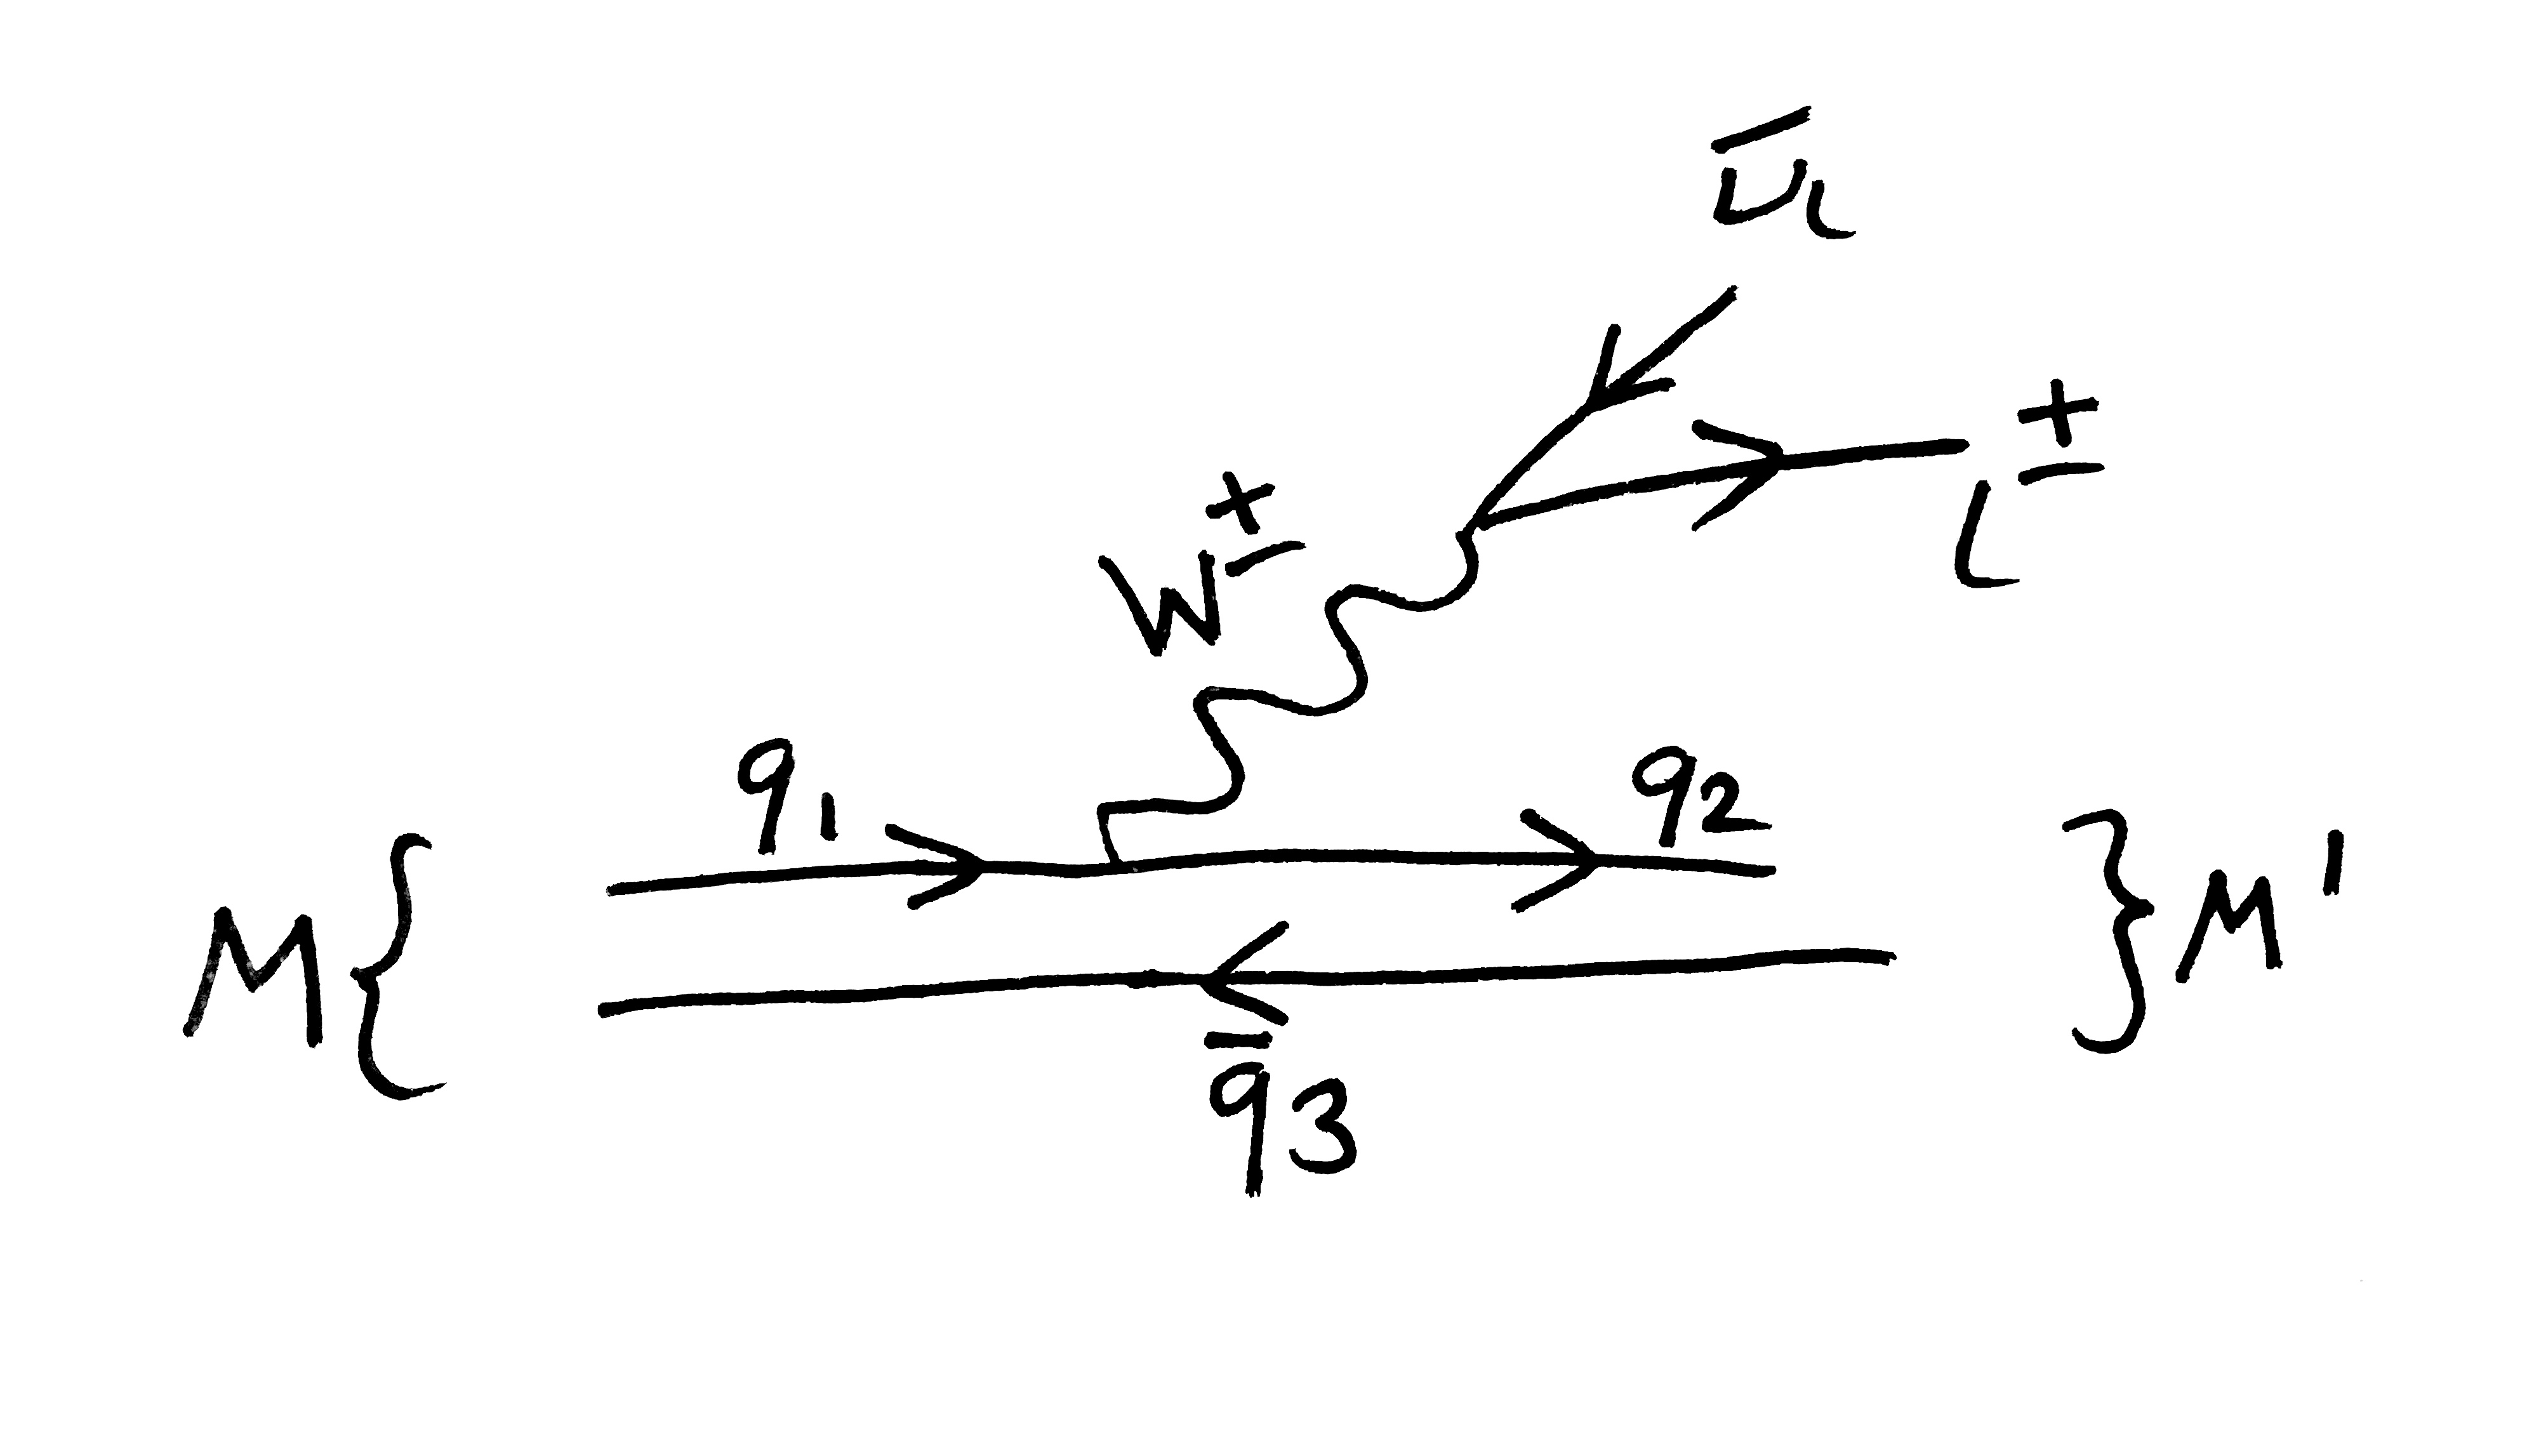
\includegraphics[width=0.6\textwidth]{images/semileptonicdecay.jpg}
  \end{center}
  \vspace{-30pt}
  \caption{Semileptonic decay, $M\to M'l\bar{\nu}$, at tree level in electroweak coupling.}
  \label{fig:semileptonicdecay}
\end{figure}
%\end{wrapfigure}

A similar story accompanies semileptonic decays. At tree level in the electroweak coupling, a typical semileptonic decay is depicted in fig. \ref{fig:semileptonic}. The amplitude is given by
\begin{align}
  \nonumber
  \mathcal{M} & = \left( { ie \over \sqrt{2} \sin\theta_W }\right) V_{q_1q_2} \langle M', l\bar{\nu} | J_{\mu}^{q_1q_2} D_W^{\mu\nu} L^l_{\nu} | M \rangle \\
  \nonumber
  & \simeq -2\sqrt{2} G_F V_{q_1q_2} \langle M', l\bar{\nu} | J_{\mu}^{q_1q_2} L^{l\, \mu} | M \rangle \\
  & \simeq -2\sqrt{2} G_F V_{q_1q_2} \langle l\bar{\nu} | L^{l\,\mu} | \Omega \rangle \langle M' | J_{\mu}^{q_1q_2} | M \rangle,
  \label{eq:semileptonic}
\end{align}
where on the second line we have integrated out the $W$ propagator in using the same expansion as in the leptonic case, and on the third line we have factorised the QCD part from the electroweak part. The matrix element $\langle M' | J_{\mu}^{q_1q_2} | M \rangle$ is a non-perturbative quantity. Unlike in the previous case, there are a number of ways one can choose to parameterise this matrix element, and appropriate choices vary depending on the quantum numbers of $M$ and $M'$. Of interest to us are the cases where $M$ is a pseudoscalar meson $0^-$, and $M'$ is either pseudoscalar or vector $1^-$.

In the {\bf{pseudoscalar$\to$pseudoscalar}} case, only the vector component of the current survives in the matrix element, $\langle M' | J_{\mu}^{q_1q_2} | M \rangle = \langle M' | V_{\mu}^{q_1q_2} | M \rangle$. $\,\,\langle M' | A_{\mu}^{q_1q_2} | M \rangle$ vanishes since this does not respect the parity invariance of QCD. The most popular parameterisation of $\langle M' | V_{\mu}^{q_1q_2} | M \rangle$ is
\begin{align}
  \langle M' | V_{\mu}^{q_1q_2} | M \rangle = f_+(q^2) \left[ P_{\mu} + p_{\mu} - {M^2-m^2\over q^2} q_{\mu} \right]  + f_0(q^2) {M^2-m^2\over q^2} q_{\mu}.
  \label{eq:formfactors_experimental}
\end{align}
$M,P_{\mu}$ are the $M$-meson mass and momentum, $m,p_{\mu}$ are the$M'$-meson mass and momentum. $f_0(q^2)$ and $f_+(q^2)$, known as the scalar and vector form factors, encoding all non-perturbative information. We now have non-perturbative functions of $q^2$ rather than a single number. $q^2=(P-p)^2$, the momentum carried away from the meson by the $W$, has an allowed range of values if the final states are on-shell;
\begin{align}
  m_l^2 \leq q^2 \leq (M-m)^2.
\end{align}
By integrating $|\mathcal{M}|^2$ over all final lepton and neutrino momenta, one finds a differential decay rate,
\begin{align}
  {d\Gamma\over dq^2}(M\to M'l\bar{\nu}) =& \eta_{\text{EW}} { G_F^2 |V_{q_1q_2}|^2\over 24 \pi^3 M^2 } \left( 1 - {m_l^2\over q^2}\right)^2 |{\bf{p}}| \,\,\times \\
  \label{eq:branchingfraction}
  &\left[ \left( 1 + {m_l^2\over 2q^2}\right) M^2 |{\bf{p}}|^2 f_+^2(q^2) + {3m_l^2\over 8q^2} (M^2-m^2)^2 f_0^2(q^2) \right]. \nonumber
\end{align}
$\eta_{\text{EW}}$ is the electroweak correction, due to diagrams involving an exchange of a photon or a $Z$-boson alongside the $W$ between the meson and leptons. ${\bf{p}}$ is the final meson state ($M'$) spacial momentum. Once again, to deduce $|V_{q_1q_2}|$, one requires both the decay rates $d\Gamma/dq^2$, and the form factors $f_0(q^2)$,$f_+(q^2)$. To precisely determine the form factors requires a Lattice QCD calculation.

In the {\bf{pseudoscalar$\to$vector}} case, both the vector and axial-vector components of the current survive in the matrix element. A common choice of parameterisation is
%% \begin{align}
%%   \langle M' | V^{\mu} | M \rangle &= {2iV(q^2)\over M+m} \epsilon^{\mu\nu\rho\sigma} \epsilon_{\nu}^* p_{\rho}P_{\sigma} \\
%%   \langle M' | A^{\mu} | M \rangle &= 2mA_0(q^2) {\epsilon^*\cdot q\over q^2} q^{\mu} + (M+m)A_1(q^2)\left[ \epsilon^{*\,\mu} - {\epsilon^*\cdot q\over q^2} q^{\mu} \right] \\
%%   \nonumber
%%   &- A_2(q^2) {\epsilon^*\cdot q\over M + m} \left[ P^{\mu} + p^{\mu} - {M^2-m^2\over q^2} q^{\mu} \right].
%% \end{align}
\begin{align}
  \langle M'(\epsilon)| V_{q_1q_2}^{\mu} | M \rangle &= i \sqrt{Mm}\, h^s_V(w) \epsilon_{\mu\nu\alpha\beta} \,\epsilon^{*\nu} v'^{\alpha} v^{\beta}, \\
  \langle M'(\epsilon)| A_{q_1q_2}^{\mu} | M \rangle &= \sqrt{Mm} \, [ h^s_{A_1}(w) (w+1) \epsilon^*_{\mu} - \\ \nonumber
    h^s_{A_2}(w)& \,\epsilon^*\cdot v \,v_{\mu} - h^s_{A_3}(w) \,\epsilon^*\cdot v \, v'^{\mu} ].
\end{align}
$v = P/M$ and $v' = p/m$ are the 4-velocities of $M$ and $M'$ respectively. $\epsilon$ is the polarization of the vector meson $M'$. $w = v\cdot v'$ is known as the recoil parameter, this is an alternative to $q^2$ often used in heavy quark effective theory. $h_V(w),h_{A_0}(w),h_{A_1}(w)$, and $h_{A_2}(w)$ are the form factors accounting for the non-perturbative physics. The decay rate is given by
\begin{align}
  {d\Gamma \over dw}(M\to M' l\bar{\nu}) = {G_F^2 m^3 | \eta_{\text{EW}} V_{q_1q_2} |^2 \over 4\pi^3 } (M-m)^2 \sqrt{w^2-1} \, \chi(w) |\mathcal{F}(w)|^2,
\end{align}
where $\mathcal{F}(w)$ is a linear combination of the form factors and $\chi(w)$ is a known function of $w$ (both given in e.g. \cite{Aubert:2006cx}).

At the zero recoil point, where $q^2$ is maximized at $q^2_{\text{max}} = (M-m)^2$, (correpsonding to $w=1$), a single form factor contributes
\begin{align}
  \mathcal{F}(1) = h_{A_1}(1).
\end{align}
However the differential decay rate vanishes at $w=1$. A common approach to determine $|V_{q_1q_2}|$, for example used to find $|V_{cb}|$ via the $B\to D^*l\bar{\nu}$ decay, is to find $|\mathcal{F}(1)V_{cb}|^2$ at zero recoil by extrapolating from experimental data at non-zero recoil, and combining this with a lattice QCD determination of $h_{A_1}(1)$.

\subsection{$b\to c$ Transitions and $|V_{cb}|$}

The family of weak decays that have attracted the most attention are decays of $B$ mesons (pseudoscalar mesons containing a valence $b$ and $u,d,s$ or $c$ quark). $B$ mesons decay into a rich variety of decay products. It is the heaviest quark flavour that can be found in hadrons (the only heavier quark, the top quark, has a mass far above the confinement scale, so does not feature as a valence quark in hadrons).

The $b$ can decay into either a $c$ or a $u$ quark via the flavour changing charged current. In this thesis we are interested in the $b\to c$ transition, with an amplitude proportional to the CKM element $|V_{cb}|$. In this section, we give a brief overview of how this is calculated and the value's current status.

$B$ meson decays can be measured in a number of experiments. There are two so-called $b$-factories, the Belle (II) experiment at the KEKB collider in Japan, and the BaBar experiment at the PEP-II collider at SLAC laboratory in the US. These are $e^+e^-$ colliders, that collide with an energy tuned to the mass of the $\Upsilon(4s)$, an excited state of the $\Upsilon$ meson (a $1^-$ state with $\bar{b}b$ valence quarks). The $\Upsilon(4s)$ has a large branching fraction into a $B\bar{B}$ pair, the decays of these can be measured with large statistics. $B$ decays can also be measured in proton colliders, like at the LHCb experiment at CERN. Measurements from LHCb have poorer statistics but cover a larger range of the phase space of final states, due to the variance of momenta in the initial state protons.

So far 3 approaches to determining $|V_{cb}|$ have been carried out:
\begin{itemize}
\item
  $B\to D^* l\bar{\nu}$ decay rate measurements are extrapolated to zero recoil to determine $|V_{cb}h_{A_1}(1)|$. Then dividing out $h_{A_1}(1)$ from a Lattice calculation, one finds $|V_{cb}|$.
\item
  $B\to D l\bar{\nu}$ decay rates are measured throughout $q^2$, and combined with $f_0(q^2)$ and $f_+(q^2)$ from lattice calculations.
\item
  $B\to X_c l\bar{\nu}$ decay rates are measured (where $X_c$ is all possible charmed final state mesons), this is used to constrain elements in the operator product expansion, a method first devised in \cite{Bigi:1996si,Hoang:1998hm}.
\end{itemize}
The first two are referred to as {\it{exclusive}} and the third {\it{inclusive}}. A selection of the most accurate examples of each method of determination is given in figure \ref{fig:Vcb_plot}.
\begin{figure}
  \vspace{-10pt}
  \begin{center}
    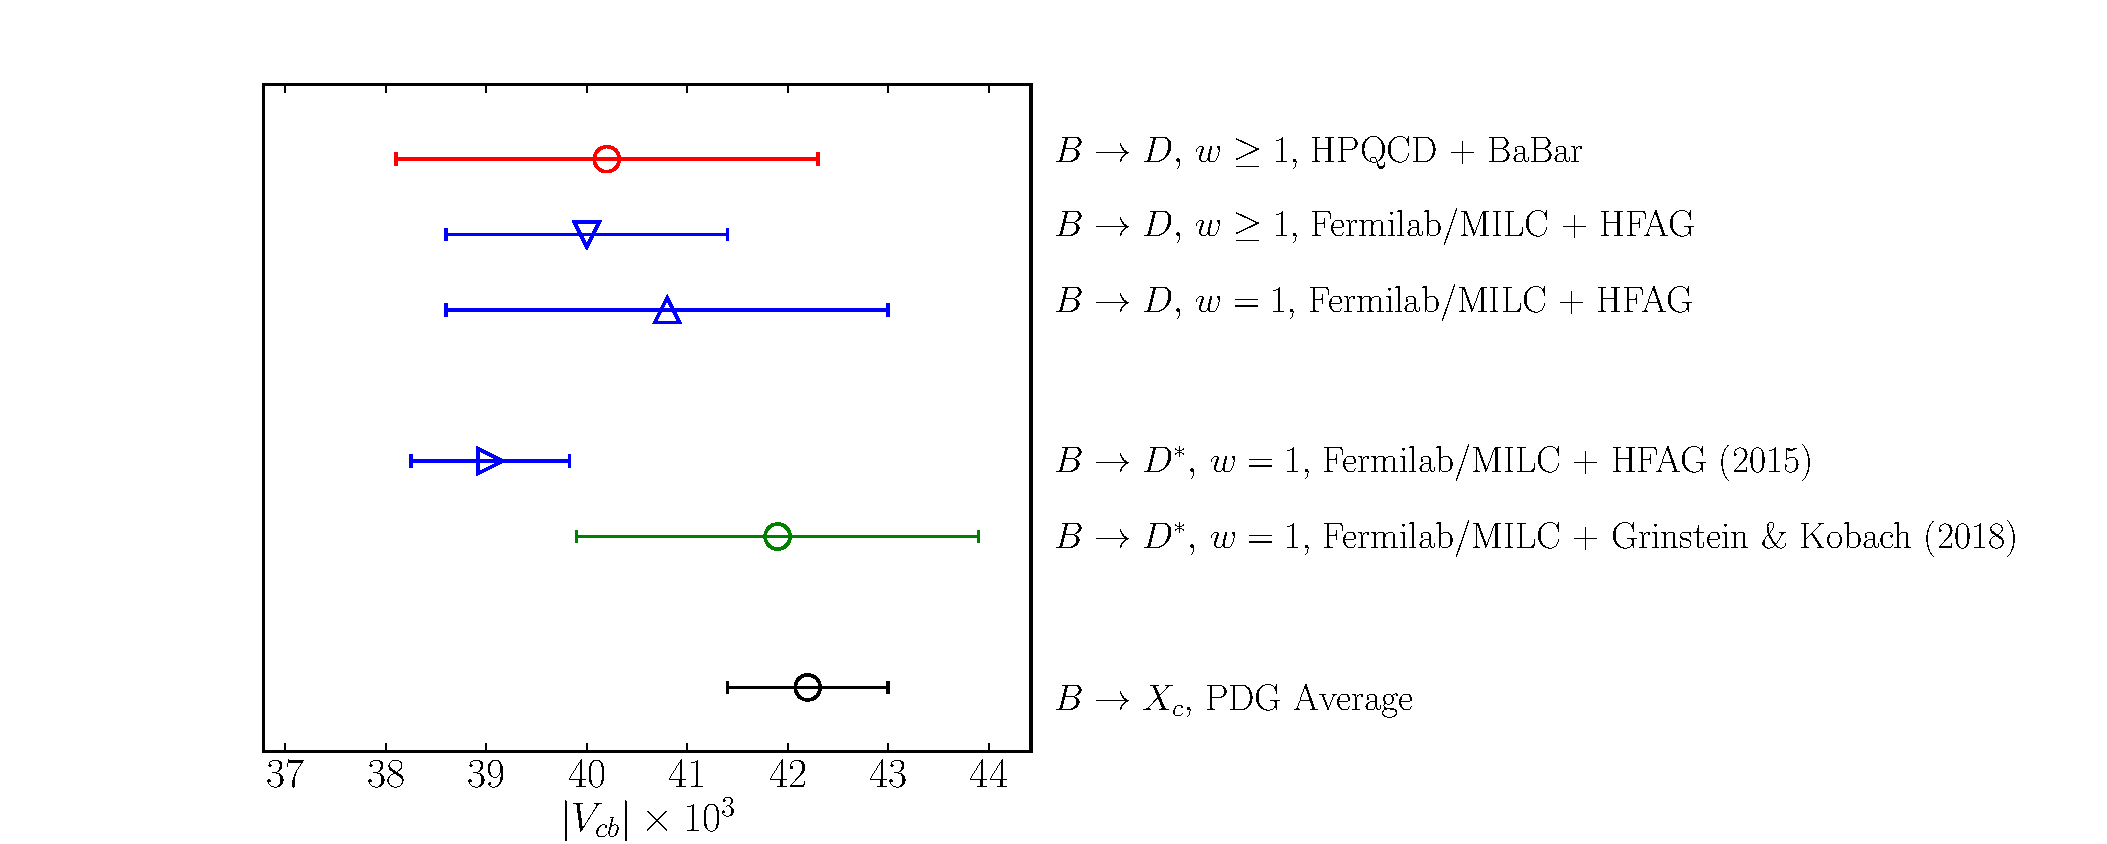
\includegraphics[width=1.0\textwidth]{images/Vcb_plot.pdf}
  \end{center}
  \vspace{-20pt}
  \caption{Different determinations of $|V_{cb}|$. Points labelled $w=1$ are determinations from extrapolating measurements of decay rates to the zero recoil point, and combining them with a lattice determination of the form factor at zero recoil. Points labelled $w\geq 1$ are results from using a combination of both branching fractions and lattice form factors through some range of $w$. The first name mentioned in the labels give the source of the lattice form factors, and the second gives the source of the experimental data (e.g. the HPQCD$+$BaBar point used form factors from the HPQCD collaboration and data from the BaBar experiment). The highest point is from \cite{Na:2015kha}, the second and third highest from \cite{Lattice:2015rga}, fourth from \cite{Bailey:2014tva}, fifth from \cite{Grinstein:2017nlq}. The bottom point is from the PDG \cite{PhysRevD.98.030001}, using data from the ALPEPH \cite{BUSKULIC1995236}, Belle \cite{Abe:2001yf}, BaBar \cite{Aubert:2008yv,Aubert:2009ac}, and CLEO \cite{Bartelt:1998dq} experiments.
    \label{fig:Vcb_plot}}
\end{figure}

This figure tells a story of the recent history of $|V_{cb}|$. Determinations from $B\to Dl\nu$ have been consistent but not as precise as via the other two methods. Until recently, there was a $3\sigma$ tension between determinations from the $B\to D^* l\nu$ decay and inclusive decays. This was on it's the way to being resolved when concern was raised about the method of extrapolating experimental data for $B\to D^*l\bar{\nu}$ decay rates to the zero recoil point ($w=1$).

The Heavy Flavour Averaging Group HFAG (Now HFLAV) determination of $|V_{cb}h_{A_1}(1)|$ in 2015 parameterised the form factors in the extrapolation using the CLN parameterisation (defined in section {\red{?}}). It has become clear that the constraints the CLN parameterisation imposes on the form factors are not justified. In \cite{Bigi:2017njr,Grinstein:2017nlq}, the results of an extrapolation using the CLN parameterisation were compared to results from a more general, model-independent parameterisation, the BGL parameterisation. It was found that they differed by $3.5\sigma$. Since the BGL makes fewer assumptions, one may consider this the more reliable result.

The $|V_{cb}|$ result using BGL to extrapolate the decay rates is given in the green point on fig. \ref{fig:Vcb_plot}. Hence, if this work is to be trusted, the long-standing $|V_{cb}|$ tension has been resolved.

There are however a number of other reasons to be interested in studying $|V_{cb}|$, namely improving its precision. It is currently the least precisely determined element of the CKM matrix. It constrains one side of the unitarity triangle via the ratio $|V_{ub}|/|V_{cb}|$, so it is the bottleneck for precise tests of CKM unitarity. It is also a dominant uncertainty in the determination of the $CP$-violation parameter $\epsilon_K$ (that is currently at tension between the SM and experiment, see for example \cite{Bailey:2018feb} where a $4\sigma$ tension is reported).

%% A dominant motivation for the work presented in this thesis is the quest for a more precise determination of $|V_{cb}|$. The main results are form factors for $B_s\to D_s l\bar{\nu}$ and $B_s\to D_s^* l\bar{\nu}$. The benefit of these determinations is two-fold. Firstly, they can be combined with future experimental measurements of $B_s\to D_s^{(*)}l\bar{\nu}$ decays for a new $|V_{cb}|$ determination. Increasing the number of independent determinations of $|V_{cb}|$ makes each result more robust. Secondly, they demonstrate that our approach in the lattice calculations work well and can, therefore, be applied to $B\to Dl\bar{\nu}$ and $B\to Dl\bar{\nu}$ form factors in the future.

\subsection{Flavour Anomalies \& Lepton Flavour Violation}

The SM can be tested by studying semileptonic decays more directly, without any consideration of CKM elements. CKM-independent observables can be constructed by taking ratios of branching fractions for decays with common CKM dependence. Then, form factors from lattice QCD can be used to form pure SM predictions of these ratios, and compared to purely experimental measurements. Such comparisons have uncovered a number of tensions between the SM and experiment.

The ratios are defined by
\begin{align}
  R_{X_q} = {\Gamma(B_q\to X_q \tau \nu_{\tau}) \over {1\over 2}\left[\Gamma(B_q\to X_q e \nu_e) + \Gamma(B_q\to X_q \mu \nu_{\mu}) \right]},
\end{align}
where $X_q$ is any meson with valence quark content $x\bar{q}$. The numerator and denomenator will have the same power of $|V_{bx}|$, so cancel in the ratio.

There is currently tension between SM and experiment in $R_D$ and $R_{D^*}$.
\begin{gather}
  R_{D^*}|_{\text{exp}} = 0.306(13)_{\text{stat}}(07)_{\text{sys}}\quad,\quad R_{D^*}|_{\text{SM}} = 0.252(3)
  \\
  R_D|_{\text{exp}} = 0.407(39)_{\text{stat}}(24)_{\text{sys}}\quad,\quad R_D|_{\text{SM}} = 0.300(8).
\end{gather}
The expermental values are the HFLAV averages, from BaBar \cite{Lees:2012xj,Lees:2013uzd}, Belle \cite{Huschle:2015rga,Sato:2016svk,Hirose:2016wfn,Hirose:2017dxl}, and LHCb \cite{Aaij:2015yra,Aaij:2017uff,Aaij:2017deq} data. The $R_{D^*}|_{\text{SM}}$ number is from \cite{Fajfer:2012vx}. $R_D|_{\text{SM}}$ is an average of Lattice results from the HPQCD \cite{Na:2015kha} and FNAL/MILC collaborations \cite{Lattice:2015rga}.

A joint analysis of $R_D$ and $R_{D^*}$ by HFLAV shows the combined tension to have a significance of $4.0\sigma$ (see fig. \ref{fig:ratiotension}). Clearly more precise experimental results are necessary to either confirm or dismiss this anomaly. While the SM values are currently much more precise than the experimental ones, further work on the theoretical results is necessary. More independent calculations are required to make the SM numbers more robust, so that, if this tension ever hits $5\sigma$, we can be confident that it is due to new physics.

\begin{figure}
  \begin{center}
    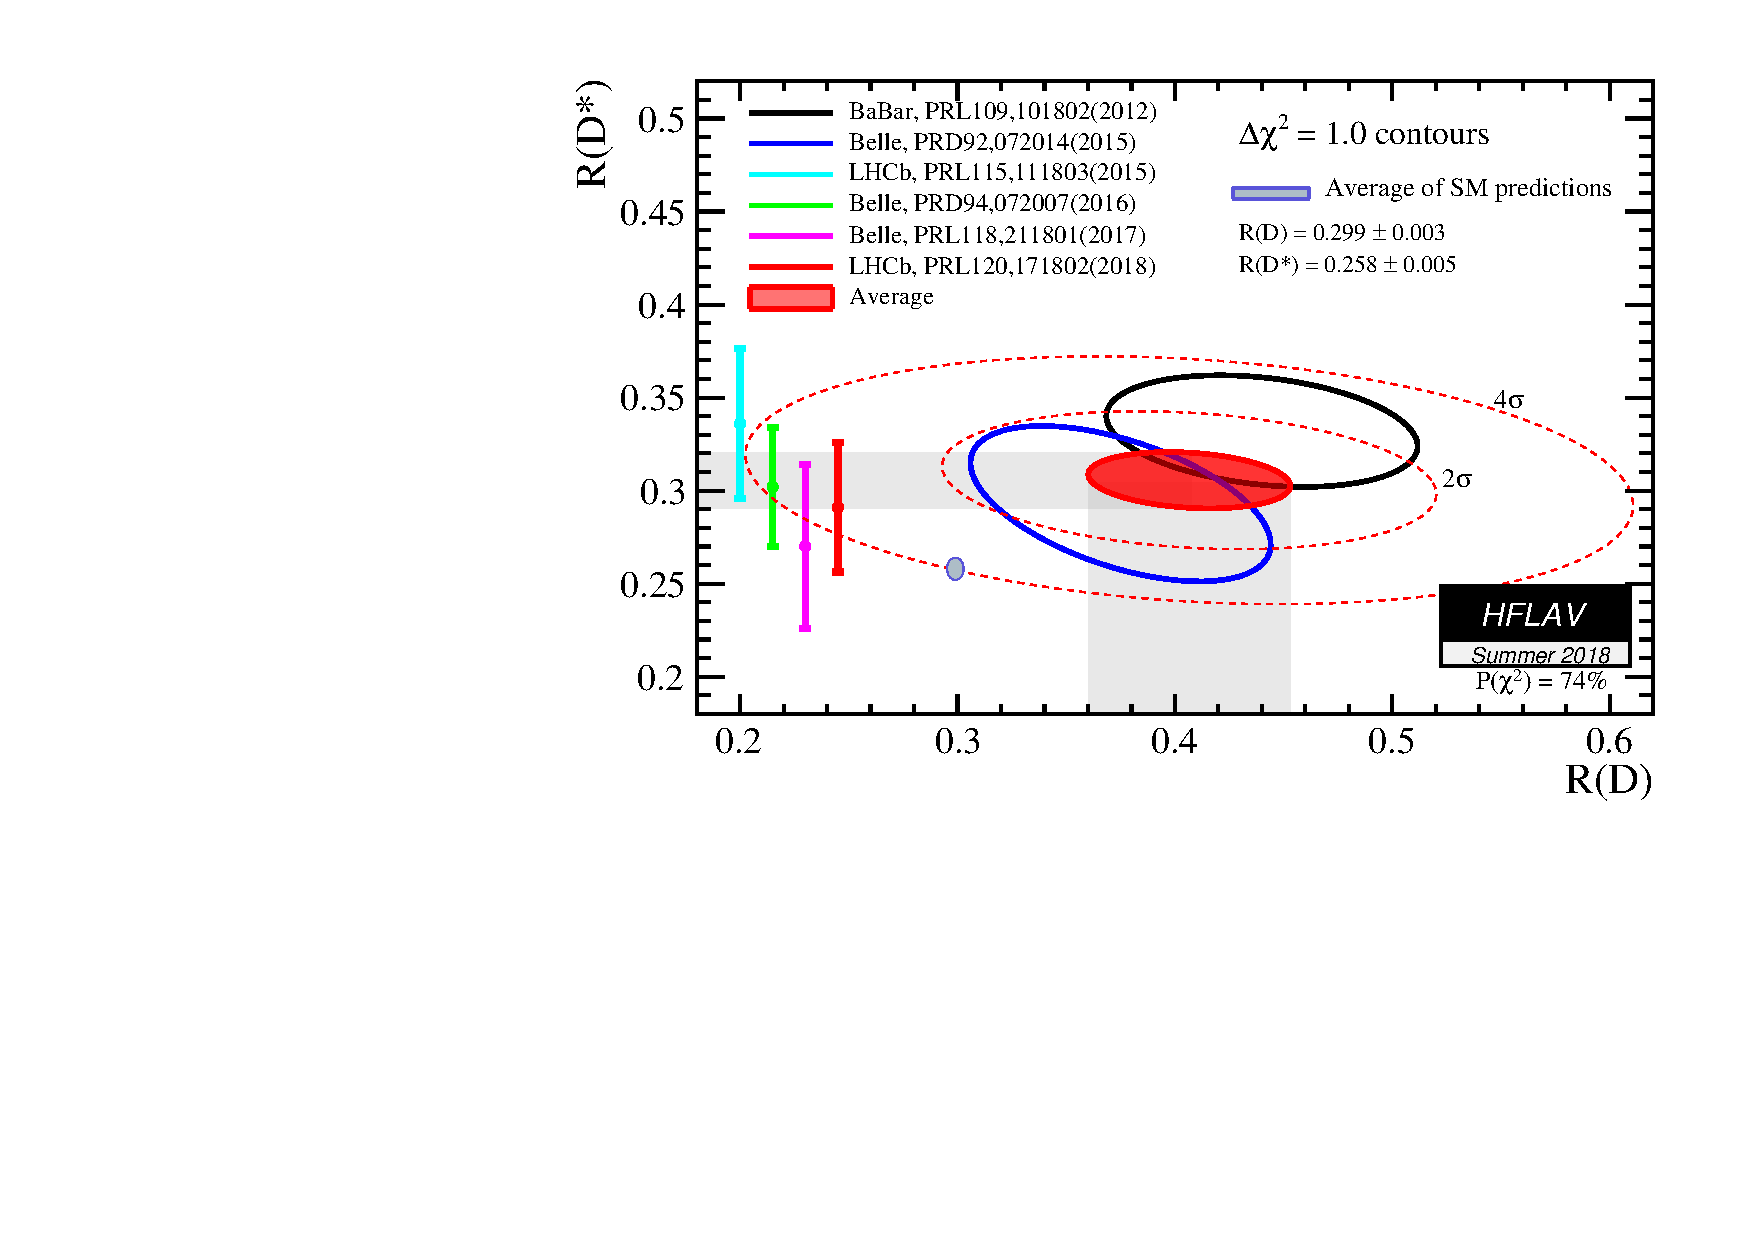
\includegraphics[width=
      0.8\textwidth]{images/rdrds_summer18.pdf}
  \end{center}
  \caption{$R(D^{(*)})$ determinations from SM and measurement
    \cite{HFLAV16}
    \label{fig:ratiotension}}
\end{figure}

There are also tensions in the quantitites \cite{Altmannshofer:2017yso}
\begin{align}
  R_{K^{(*)}} = {\Gamma( B\to K^{(*)}\mu^+\mu^-)\over \Gamma( B\to K^{(*)} e^+e^-)}.
\end{align}
LHCb measured $R_K$ between 1 and 6GeV, and found a disagreement with the SM value \cite{Bobeth:2007dw,Bouchard:2013mia} of 2.6$\sigma$ \cite{Aaij:2014ora}. LHCb also measured $R_{K^*}$ in 2 bins ($0.045<q^2<1.1 $GeV$^2$ and $1.1<q^2<1.6$GeV$^2$), and reported disagreement with the SM prediction \cite{Bordone:2016gaq,Descotes-Genon:2015uva,Capdevila:2016ivx,Capdevila:2017ert,Serra:2016ivr,Straub:2015ica,Altmannshofer:2017fio,Jager:2014rwa} of 2.1-2.3$\sigma$ and 2.4-2.5$\sigma$ respectively \cite{Aaij:2017vbb}.

%% A useful direction we could go in, besides improving the precision of these ratios, is to test other ratios where LFV should show up. For example, in this thesis, we provide a new prediction of $R_{D_s}$, which when combined with future experimental data, will help eludicate this picture.

Each of these anomalies points to one potential new physics scenario: lepton flavour violation (LFV), a breakdown of the lepton flavour universality in the SM discussed in Sec. \ref{sec:fccc}. A consequence of LFV would be that the different leptons generations would no longer have the same coupling to gauge fields. For example, imagine couplings like $U_{ij} \bar{e}_L^i \slashed{W}^+ \nu_L^j$, where $U_{ij}$ is unitary but non-diagonal, then the different lepton generations would have different couplings to $W$. This can lead to a modification of the $B\to D^{(*)}l\nu$ and $B\to K^{(*)}\bar{l}l$ decays rates by different amounts depending on the lepton flavours in the final state, resulting in the ratios $R_{D^{(*)}}$, $R_{K^{(*)}}$ deviating from the SM prediction.

There are broadly speaking two ways one can explain LFV. The first is to posit that there are in fact right-handed neutrinos, $\nu_R$, and neutrinos have Dirac mass terms $m\bar{\nu}_L\nu_R$, from their coupling with the Higgs, just like the charged leptons and quarks. Then, the argument preventing the presence of non-trivial lepton flavour structure in $\mathcal{L}_{\text{FCCC}}$ breaks down, we obtain an equivalent of the CKM matrix for leptons (the Pontecorvo-Maki-Nakagawa-Sakata (PMNS) matrix), and lepton flavour violation is mediated by the $W$. Neutrinos have in fact already been shown to have mass, the PMNS matrix exists, and it's elements have been measured. However, as mentioned already, these effects would be extremely small due to the extreme lightness of the neutrinos. Experiments have looked for evidence of $W$-mediated LFV processes, $\tau\to \mu\gamma$ and $\mu\to e\gamma$, and they found upper bounds for their branching fractions of $4.2\times 10^{-13}$ \cite{Abe:2003sx} and $3.1\times 10^{-7}$ \cite{TheMEG:2016wtm} respectively.

Besides there being no evidence for $W$-mediated LFV, this picture of neutrino masses is not very aesthetically satisfying. It requires unnaturally small Yukawa couplings between the Higgs and the neutrinos. The second, and much more popular approach, to explaining both LFV and neutrino masses, is the presence of new physics.

In the face of evidence against the SM, the most general way to parameterise the space of possible new physics models is to study the Standard Model Effective Theory (SMEFT). In this approach, one introduces a higher dimension, non-renormalisable operators to the standard model (the SM has only renormalisable dimension 4 operators), and impose a hard momentum cutoff $\Lambda$. Then, the SMEFT is
\begin{align}
  \mathcal{L}_{\text{SMEFT}} = \mathcal{L}_{\text{SM}} + \sum_i {c^{(5)}_i\over\Lambda} \mathcal{O}^{(5)}_i + \sum_i {c^{(6)}_i\over\Lambda^2} \mathcal{O}^{(6)}_i + ...
\end{align}
where $\mathcal{O}_i^{(d)}$ is the set of dimension-$d$ operators that satisfy the symmetries of the SM, and $c_i^{(d)}$ are coefficients to be measured, known as Wilson coefficients. Wilson coefficients differing from the SM expectation can be evidence that the SM must be augmented with new fields at energies above $\Lambda$, and the quantum numbers of the associated operators gives information about the quantum numbers of the new fields.

One can fit the avaliable $B\to D^{(*)}l\bar{\nu}$ and $B\to K^{(*)}\bar{l}l$ data to predictions from SMEFT, in order to infer the Wilson coefficients neccesary to explain the anomalies. In \cite{Freytsis:2015qca} it was found that $R_{D^{(*)}}$ can be explained with the $d=6$ operators
\begin{gather}
  \nonumber
  (\bar{c}\gamma_{\mu}P_L b)(\bar{\tau}\gamma^{\mu} P_L \nu_{\tau}), \quad
  (\bar{c}\sigma^{\mu\nu} P_L b)(\bar{\tau} \sigma_{\mu\nu} P_L \nu_{\tau}), \quad
  (\bar{\tau} P_L c^c)(\bar{b}^c P_L \nu_{\tau}), \\
  (\bar{\tau}\gamma_{\mu} P_R b) (\bar{c} \gamma^{\mu} P_L \nu_{\tau}), \quad
  (\bar{\tau}\gamma_{\mu}P_L b)(\bar{c}\gamma^{\mu} P_L \nu_{\tau}), \quad
  (\bar{\tau}P_R c^c)(\bar{b}^c \gamma^{\mu} P_L \nu),
\end{gather}
where $P_{L/R} = (1\pm \gamma_5)/2$, $\psi^c = -i(\bar{\psi}\gamma^0\gamma^2)^T$ and $\bar{\psi}^c = -i(\gamma^0\gamma^2 \psi)^T$. In \cite{Altmannshofer:2017yso}, a similar process found the operators neccesary to explain $R_{K^{(*)}}$:
\begin{gather}
  \nonumber
  (\bar{s}\gamma_{\mu}P_L b)(\bar{e}\gamma^{\mu}e), \quad (\bar{s}\gamma_{\mu}P_L b)(\bar{\mu}\gamma^{\mu}\mu) \\
  (\bar{s}\gamma_{\mu}P_L b)(\bar{e}\gamma^{\mu}\gamma_5e), \quad (\bar{s}\gamma_{\mu}P_L b)(\bar{\mu}\gamma^{\mu}\gamma_5\mu)
\end{gather}
This information, along with constraints from other measurements, strongly reduces the space of possible new physics models that could produce these anomalies. Hot topics include Leptoquarks, $Z'$ models, and partial compositeness \cite{Altmannshofer:2017yso,Freytsis:2015qca,Bauer:2015knc,Crivellin:2015mga}.



%%%%%%%%%%%%%%%%%%

\section{Strong Interaction Physics}
\label{sec:stronginteractions}

The work of this thesis is essentially quantifying the effect the strong interaction has on branching fractions for semileptonic decays. The strong interaction and the observed pattern of hadrons can be explained with Quantum Chromodynamics (QCD). In this section we review the fundamental theory, and the force's physical features.

\subsection{Quantum Chromodynamics}
\label{sec:qcd}

QCD is an $SU(3)$ Yang-Mills gauge theory. The Lagrangian is derived by requiring:
\begin{itemize}
\item
  $N_f$ fermion fields transforming in the fundamental representation of the $SU(3)_C$ gauge group.
\item
  Invariance under that gauge group.
\item
  Renormalizability of all interactions.
\end{itemize}
From these we find \cite{Schwartz:2013pla}
\begin{align}
  \mathscr{L}_{\text{QCD}} &= \sum_i \bar{q}_i (i \slashed{D} - m_i) q_i - {1\over 4} \text{Tr}G_{\mu\nu} G^{\mu\nu} - g{\bar{\theta}\over 64 \pi^2} \epsilon^{\mu\nu\rho\sigma} \text{Tr}G_{\mu\nu} G_{\rho\sigma} \\
  &D_{\mu} = \partial_{\mu} - i g G_{\mu} \,,\quad
  G_{\mu\nu} = [ D_{\mu}, D_{\nu} ].
  \nonumber
\end{align}
$q_i = ( q_{i,r}, q_{i,b}, q_{i,g} )$ are the $N_f$ fermions, vectors in {\it{color space}}, transforming under
\begin{align}
  q_i(x) \to \Lambda(x)q_i(x) \,,\, \bar{q}_i(x) \to \bar{q}_i(x) \Lambda^{\dagger}(x),
  \label{eq:quark_gauge_trans}
\end{align}
where $\Lambda(x)$ is an $SU(3)$ matrix acting on color the color space. $G_{\mu}$ are the $\mathfrak{su}(3)$-valued gluon fields, transforming under the Gauge group like
\begin{align}
  G_{\mu}(x) \to \Lambda(x) G_{\mu}(x) \Lambda^{\dagger}(x) - {i\over g} [ \partial_{\mu} \Lambda(x) ] \Lambda^{\dagger}(x).
  \label{eq:G_gauge_trans}
\end{align}
$g$ is the coupling constant of the theory, often expressed instead as $\alpha_s = (g/4\pi)^2$. $\bar{\theta}$ has strong experimental bounds on it's size, to the extent that for our purposes it can be neglected \cite{ALTAREV1992242}.

The most notable feature of QCD is due to the running of the QCD coupling $\alpha_s$ \cite{PhysRevLett.30.1343}.
\begin{figure}
  \begin{center}
    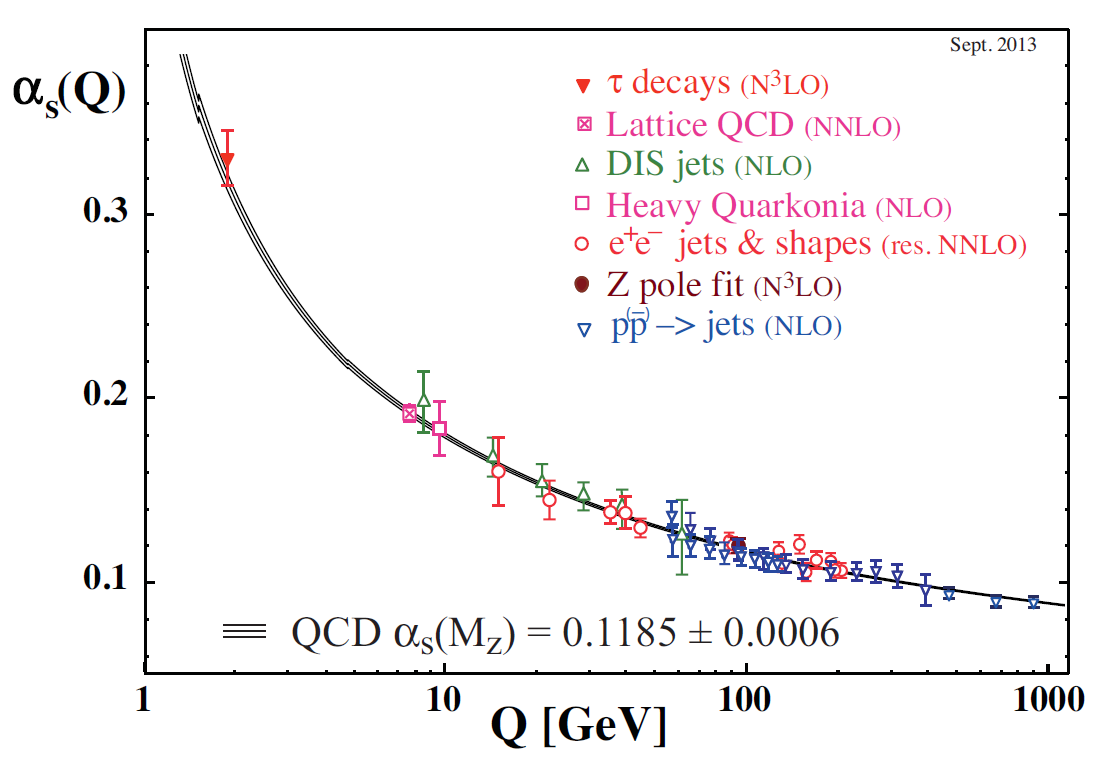
\includegraphics[width=0.7\textwidth]{images/QCD-running-coupling.png}
  \end{center}
  \caption{The relationship between scale $Q$ and the strong coupling constant $\alpha_s$, from the PDG \cite{PhysRevD.98.030001}.}
  \label{fig:semileptonic}
\end{figure}
In contrast with the electroweak force, the coupling of the strong force diverges at low energies. This is referred to as {\it{asymptotic freedom}}. At energies around or below $\Lqcd \sim 0.5$GeV, $\alpha_s$ becomes too large to be a good expansion parameter, and perturbation theory becomes unreliable for making predictions.

At large $\alpha_s$, quarks and gluons become strongly interacting, this is believed to be the source of confinement, the mechanism that bounds quarks together into hadrons. %A common assumption then is that all of the dynamics that occur inside hadrons have energies on the scale of $\Lqcd$.

Broadly speaking there are two approaches to QCD at low energies:
\begin{enumerate}
\item
  Chiral Perturbation theory - an effective theory of hadrons with the same symmetry properties as QCD.
\item
  Lattice simulations - solve the path integral by brute force, eliminating the need for an expansion in $\alpha_s$. This is covered in chapters \ref{chap:latticeqcd} and \ref{chap:latticecalculations}, since it is the method used in the work presented in this thesis.
\end{enumerate}

\subsection{Chiral Symmetry}
\label{sec:chiralsymmetry}

In the limit of $m_i\to 0\,\,\forall i$, QCD develops two new global symmetries between the flavours;
\begin{align}
  \label{eq:vector_chiral}
  q_i &\to \exp(i\theta_a \lambda^{ij}_a) q_j \\
  q_i &\to \exp(i\gamma_5 \theta_a \lambda^{ij}_a) q_j
\end{align}
where $\lambda_a$ are $U(N_f)$ matrices. They are labelled $U(N_f)_V$ and $U(N_f)_A$ respectively, standing for vector and axial-vector.
% Each of these groups can be decomposed into $U(1)_{V/A}\times SU(N_f)_{V/A}$, the $U(1)$ contains the single element corresponding to $\lambda_a=1$, and $SU(N_f)$ contains the elements where $\lambda_a$ are $SU(N_f)$ generators. Neccesary?

Via Noether's theorem, these symmetries imply currents that are conserved in the massless limit \cite{Scherer:2002tk};
\begin{align}
  \label{eq:chiralcurrents}
  V_{\mu}^a = \bar{q} \gamma_{\mu} \lambda_a q \quad,\quad
  A_{\mu}^a = \bar{q} \gamma_{\mu} \gamma_5 \lambda_a q
\end{align}

The way in which the chiral symmetry is realised in quantum mechanics is captured by the {\it{Ward identities}}. There is an infinite number of possible Ward identities, but for the purpose of our work, we only need to consider the most simple of them. %We will derive these below.

Consider the partition function for QCD:
\begin{align}
  \mathcal{Z} = \int [d\psi d\bar{\psi} dA] e^{iS[\psi,\bar{\psi},A]},
\end{align}
where $[d\psi d\bar{\psi} dA]$ represents the functional integral over qark,antiquark and gauge fields. Consider performing a shift of the integration variables of the form \eqref{eq:vector_chiral}, and allow the parameters $\theta_a$ to be local, $\theta_a=\theta_a(x)$. The partition function becomes
\begin{align}
  \mathcal{Z} = \int \mathcal{J} [d\psi d\bar{\psi} dA] ( 1 + i\delta S ) e^{iS[\psi,\bar{\psi},A]}
  \label{eq:partition_transformed}
\end{align}
%$\mathcal{J}$ is the Jacobian of the measure $[d\psi d\bar{\psi} dA]$ under the coordinate transform \eqref{eq:vector_chiral}. In many cases, this will be non-trivial, even if the transform is classically a symmetry of the theory. This can be due to a regularization of the path integral that does not respect the symmetries of the theory. Alternatively, it could be due to an anomaly - an instance of a classical symmetry not holding in quantum mechanics. The symmetries we will be concerned with in this work will always be anomaly-free, so let's set $\mathcal{J}=1$.

$\mathcal{J}$ is the Jacobian of the measure $[d\psi d\bar{\psi} dA]$ under the coordinate transform \eqref{eq:vector_chiral}. In many cases, $\mathcal{J}$ will be non-trivial, due to either regularization schemes that don't respect the symmetry or quantum anomalies. The symmetries we are concerned with here are anomaly free, so $\mathcal{J}=1$.

The effect of the local version of \eqref{eq:vector_chiral} on the action is
\begin{align}
  \delta S = \int d^4x \theta_a(x) \left[ \partial_{\mu} V_a^{\mu}(x) - i\bar{q}(x) [\lambda_a,M] q(x) \right],
\end{align}
where $M = \text{diag}(m_u,m_d,m_s,...)$ acts on flavour. Setting the arbitrary parameters $\theta_a(x)$ to $1$ and removing $\mathcal{Z}$ from each side of \eqref{eq:partition_transformed}, and removing the spacetime integral $\int d^4x$ results in
\begin{align}
  \partial_{\mu}\langle V_a^{\mu} \rangle = i \langle \, \bar{q} [ \lambda_a, M ] q \, \rangle,
  \label{eq:vector_ward}
\end{align}
where $\langle \rangle$ represents a quantum expectation value, the state the expectation value is taken need not be specified since the above derivation does not assume any particular state. Repeating the above steps with the vector chiral transform replaced with the axial-vector chiral transform, one finds
\begin{align}
  \partial_{\mu}\langle A_a^{\mu} \rangle = i \langle\, \bar{q} \{ \lambda_a,M \} q \,\rangle.
  \label{eq:axial_ward}
\end{align}
\eqref{eq:vector_ward} and \eqref{eq:axial_ward} are examples of Ward identities, they describe the non-conservation of the chiral currents.

A useful theorem \cite{Fubini:1964boa} is that partially conserved currents (currents that become conserved when some parameter in the theory vanishes, like $V^{\mu}_a$ and $A^{\mu}_a$) require no renormalisation under any regularisation scheme. %We will now demonstrate this.
The conserved or partially conserved current $J_a^{\mu}$ has a corresponding charge $Q_a(t) = \int d^3x J^{0}(\underline{x},t)$ that is the generator of it's corresponding symmetry transform on Hilbert space. In this case, these charges are members of the Lie algebra of the symmetry group;
\begin{align}
  [ Q_a(t), Q_b(t) ] = if_{abc} Q_c(t),
  \label{eq:charge_commutator}
\end{align}
where $f_{abc}$ are the structure constants of the algebra. Under some regularisation, change in regularisation scheme, or running of scale, each operator in the theory may require multiplicative renormalisations; $Q_a \to Z_Q Q_a$. Equation \eqref{eq:charge_commutator} demands that $Z_Q=1$, so $J^0$ obtains no renormalisation, and if the regularization is lorentz invariant, this carries on to $J^{\mu}$.

%% In the case of the chiral currents $V_a^{\mu},A_a^{\mu}$, the Ward identities \eqref{eq:vector_ward}, \eqref{eq:axial_ward} cause this property to carry onto the operators on the LHS, $\bar{q} [\lambda_a,M] q$ and $\bar{q} \{ \lambda_a,M \} q$, these operators receive no normalisation under any regularisation scheme.

Since one can transform any flavour into any other flavour via the chiral $U(N_f)$ generators, one can build currents charged with any combination of flavours from linear combinations of $V_a^{\mu}$ and $A_a^{\mu}$;
\begin{align}
  \label{eq:vector_ward_indiv}
  V_{ij}^{\mu} &= \bar{q}_i \gamma^{\mu} q_j \,,\quad\quad \partial_{\mu}\langle V^{\mu}_{ij} \rangle = i ( m_i - m_j ) \langle S_{ij} \rangle \\
  A_{ij}^{\mu} &= \bar{q}_i \gamma^{\mu}\gamma^5 q_j \,,\quad \partial_{\mu}\langle A^{\mu}_{ij} \rangle = i ( m_i + m_j ) \langle P_{ij} \rangle
  \label{eq:axial_ward_indiv}
\end{align}
where we have defined $S_{ij} = \bar{q}_iq_j$ and $P_{ij} = \bar{q}_i\gamma^5 q_j$, the scalar and pseudoscalar densities. The non-renormalisation of $V_a^{\mu}$ and $A_a^{\mu}$ carry on to $V_{ij}^{\mu}$ and $A_{ij}^{\mu}$, and onto the operators $( m_i - m_j ) S_{ij}$, $( m_i - m_j ) P_{ij}$ via the Ward identities.

The partially conserved currents $V^{ij}_{\mu}$ and $A^{ij}_{\mu}$ are the same currents that feature in the matrix element of leptonic and semileptonic decays in Sec. \ref{sec:fccc}, and their expectation values appear in amplitudes for leptonic and semileptonic decays. Hence, the fact that these can be related to alternative expectation values via ward identities, and that they obtain no renormalisation, is very useful in the calculation of these amplitudes.

\section{Heavy Quark Physics}

Quarks with mass $m_Q >> \Lqcd$ are referred to as heavy quarks. Charm and bottom quarks are considered heavy: $\Lqcd/m_c \sim 1/4$, $\Lqcd/m_b \sim 1/14$. This separation of scales can come in very useful. They mean one can integrate out the degrees of freedom at $m_Q$, and still have a good description of the dynamics at $\Lqcd$. This philosophy gives rise to Heavy Quark Effective Theory (HQET). We will summarise the aspects of this theory most relevant to our work.

%% The physical picture of a meson containing a heavy quark is very similar to that of a hydrogen atom. In the hydrogen atom, the nucleus has a mass much greater than the characteristic energies of the electron and photons. One can treat the nucleus as a static source of electric charge, and solve to high precision the dynamics of the electron. The electron's behaviour is not affected by the mass or the spin of the nucleus. Similarly, one can consider a heavy quark in a meson to be a static source of colour charge, and solve the $\Lqcd$ dynamics in its presence. The mass and spin of the heavy quark does not effect the light degrees of freedom, this is the well understood {\it{heavy quark symmetries}}. The effective field theories introduced in this section gives us a framework to take this approximation and systematically correct for it.

\subsection{HQET}

HQET is an effective field theory with the cutoff at the heavy quark mass $m_Q$, and terms organized in a series in $\Lambda_{\text{QCD}}/m_Q$. Since at the $b$ (and $c$) mass QCD is perturbative ($\alpha_s(m_Q) << 1$), one can match HQET to perturbative QCD at $m_Q$, then run the couplings of HQET down to produce useful predictions at the confinement scale.

%% It is a useful tool for when we perform extrapolations in heavy quark mass, as it supplies us with explicit expressions for the heavy quark mass dependence on various phenomenological quantities.

\subsubsection{HQET Lagrangian}

We will derive HQET for a single heavy quark interacting with gluons, the generalization to many flavours is straightforward. The fermion part of the Lagrangian is
\begin{align}
  \mathscr{L}_{\text{QCD}} = \bar{Q} ( i\slashed{D} - m_Q ) Q,
  \label{eq:dirac}
\end{align}
where $Q$ is the heavy quark field. Define the heavy quark velocity $v$ according to $v = p_Q/m_Q$. Split $Q$ into ``heavy'' and ``light'' components:
\begin{align}
  \label{eq:hdef}
  Q = h + H\quad : \quad &h = {1\over 2} e^{-im_Q v\cdot x} ( 1 + \slashed{v} ) Q \\
  &H = {1\over 2} e^{-im_Q v\cdot x} ( 1 - \slashed{v} ) Q
\end{align}
with the important property
\begin{align}
  \slashed{v} h = h \quad \slashed{v} H = - H.
\end{align}
In terms of these new fields the Lagrangian becomes
\begin{align}
  \mathscr{L}_{\text{QCD}} = i\bar{h} (v\cdot D) h - \bar{H} ( i(v\cdot D) - 2m_Q ) H
  + i \bar{h} \slashed{D}^{\perp} H + i \bar{H} \slashed{D}^{\perp} h.
  \label{eq:HQET_preintegral}
\end{align}
where $v_{\mu}(v\cdot D)$ is the covariant derivative projected along the direction of $v$, and $D^{\perp} = D - v_{\mu}(v\cdot D)$ are the components perpendicular to $v$. %In the rest frame of the heavy quark, $v = (1,0,0,0)$ so $v_{\mu}(v\cdot D)$ becomes the temporal derivative and $D^{\perp}$ the spacial.
A physical interpretation of the definition of $h$ in \eqref{eq:hdef} can be seen by acting a spacial derivative on the definition of $h$, and by recognising $\partial Q = -i p_Q$, $\partial h = -i p_h$, we find that
\begin{align}
  p_Q = m_Q v + p_h.
\end{align}
Since $p_h << p_Q$, we see that the quark's momentum is dominated by it's mass (the quark is close to on-shell), and the $h$ field represents perturbations around on-shell due to interactions with the lighter degrees of freedom at $\Lambda_{\text{QCD}}$.

From \eqref{eq:HQET_preintegral}, we see that $h$ is a massless field and $H$ has a mass of $2m_Q$. From this Lagrangian we can derive an equation of motion for $H$:
\begin{align}
  ( i(v\cdot D) + 2m_Q) H = i\slashed{D}^{\perp} h,
\end{align}
with the solution
\begin{align}
  H = {1\over i(v\cdot D) + 2m_Q} i\slashed{D}^{\perp} h = {1\over 2m_Q}\sum_{n=0}^{\infty} {(-i(v\cdot D))^n\over 2m_Q} \slashed{D}^{\perp} h.
\end{align}
By substituting this into the Lagrangian we arrive at
\begin{align}
  \mathscr{L}_{\text{HQET}} = i \bar{h} (v\cdot D) h - \bar{h} \slashed{D}^{\perp} {1\over 2m_Q}\sum_{n=0}^{\infty} {(-i(v\cdot D))^n\over 2m_Q} \slashed{D}^{\perp} h.
  \label{eq:HQET_lagrangian}
\end{align}
%This can be found by a more rigorous proof by performing the Gaussian integration over the $H$ field in the path integral {\color{red}{ref!}}.
Since we expect $v\cdot D \sim \Lambda_{\text{QCD}}$, we can interpret the infinite sum as a series in $\Lambda_{QCD}/m_Q$, and truncate it at some order. %For example to $\mathcal{O}(\Lambda_{\text{QCD}}/m_Q)$, we have
%% \begin{align}
%% \mathcal{L}_{\text{HQET}^1} = i \bar{h} (v\cdot D) h - {1\over 2m_Q} \bar{h} \slashed{D}^{\perp 2} h
%% \label{eq:HQET1}
%% \end{align}

Leading order HQET exhibits new symmetries not present in full QCD, known as the heavy quark symmetries. Since $m_Q$ is not present in the leading order Lagrangian, there is a flavour symmetry - a set of $N$ heavy quarks with the same $v$ can be mixed via an $SU(N)$ symmetry. Similarly, due to the absence of spin-mixing matrices, a heavy quark has an $SU(2)$ spin symmetry. This builds up a physical picture of a heavy quark in a meson being a static colour charge, the dynamics at $\Lambda_{\text{QCD}}$ are not effected by its mass or spin.

We will now use HQET to derive a useful theorem used in our work.

%% \subsubsection{Isgur-Wise Function}
%% \label{sec:isgurwise}

%% A consequence of heavy quark symmetry relevant to semileptonic decays are the Wigner-Eckart theorems. Consider a transition amplitude between two heavy pseudoscalar mesons:
%% \begin{align}
%%   \langle M(v) | \bar{h} \Gamma h | M(v') \rangle
%% \end{align}
%% The spin structure of $| M(v) \rangle$ is $\gamma_5 (1-\slashed{v})$, this can be shown with the following argument. The state can be generally written as $| M(v) \rangle = \int d^4x d^4y f(x,y) \bar{h}(x) \gamma_5 q(y) | \Omega \rangle$ where $q$ is the light valence quark and $|\Omega\rangle$ is the interacting vacuum. Using $\slashed{v} h = h$, this can be reexpressed as $| M(v) \rangle = \int d^4x d^4y f(x,y) \bar{h}(x) \gamma_5 (1-\slashed{v}) q(y) | \Omega \rangle /2$. %Then via the spin symmetry, one can always rotate the $h$ spin in the meson state such that it matches the spin of the current, i.e. $h_{\alpha} \bar{h}_{\beta} \to 1_{\alpha\beta} f(h,\bar{h})$.

%% The amplitude can be written as
%% \begin{align}
%% \langle M(v) | \bar{h} \Gamma h | M(v') \rangle = m_M \text{Tr}[ {1\over 2} \gamma_5 (1 - \slashed{v}) \Gamma {1\over 2} \gamma_5 (1 - \slashed{v'}) \mathcal{M}(v,v')]
%% \label{eq:wignereckart1}
%% \end{align}
%% where $\mathcal{M}(v,v')$ can be any gamma-matrix valued function. The $m_M$ factor comes from the relativistic normalisation of the states. A general spin decomposition of this is
%% \begin{align}
%% \mathcal{M}(v,v') = \xi_0(v\cdot v') + \slashed{v} \xi_1(v\cdot v') + \slashed{v'} \xi_2(v\cdot v') + \slashed{v}\slashed{v'} \xi_4(v\cdot v').
%% \end{align}
%% Plugging this into \eqref{eq:wignereckart1}, we can then write the amplitude in terms of a single function:
%% \begin{align}
%% \langle M(v) | \bar{h} \Gamma h | M(v') \rangle = m_M \text{Tr}[ {1\over 2} \gamma_5 (1 - \slashed{v}) \Gamma {1\over 2} \gamma_5 (1 - \slashed{v'}) ] \xi(v\cdot v'),
%% \end{align}
%% where $\xi(v\cdot v') = \xi_0(v\cdot v') + \xi_1(v\cdot v') - \xi_3(v\cdot v') - \xi_4(v\cdot v')$ is known as the Isgur-Wise function. For a general pair of mesons with spin structure $\mathcal{H}$,$\mathcal{H}'$, a transition amplitude between them with a heavy current insertion can always be written as
%% \begin{align}
%% \langle \mathcal{H} | \bar{h} \Gamma h | \mathcal{H}' \rangle = \xi(v\cdot v') Tr[ \bar{\mathcal{H}} \Gamma \mathcal{H} ] + \order{\Lambda_{\text{QCD}}\over m_Q}
%% \end{align}
%% So all heavy semileptonic decays involving any combination of masses or spins are described by a single non-perturbative function, $\xi(v\cdot v')$. Examples relevant to the work of this thesis are:
%% \begin{align}
%% \langle D(v') | \bar{c_{v'}} \gamma^{\mu} b_v | B(v) \rangle &= \sqrt{m_B m_D} ( v + v')^{\mu} \xi(v\cdot v') \\
%% \langle D^*(v') | \bar{c_{v'}} \gamma^{\mu} b_v | B(v) \rangle &= i \sqrt{m_B m_D*} \epsilon^{\mu\nu\alpha\beta} \varepsilon_{\nu}^* v'_{\alpha} v_{\beta} \xi(v\cdot v')  \\
%% \langle D^*(v') | \bar{c_{v'}} \gamma^{\mu}\gamma_5 b_v | B(v) \rangle &= \sqrt{m_B m_D*} [ \varepsilon^{*\mu}(v\cdot v' + 1) - v^{'\mu} \varepsilon^*\cdot v] \xi(v\cdot v').
%% \end{align}
%% Here we have subscripted the fields $c_{v'}$,$b_v$ to specify the velocity used to separate those fields from the heavy components e.g. in eq. \eqref{eq:hdef}.

\subsubsection{Luke's Theorem}

Luke's theorem, which can be derived from the Ademollo-Gatto (AG) theorem, tells us the leading order heavy quark mass dependence of form factors. First we will derive the AG theorem. We will follow the proof given in \cite{Lebed:1991sq}.

Consider the transition amplitude
\begin{align}
  \langle \alpha | Q_a | \beta \rangle,
\end{align}
where $Q_a$ is a conserved charge associated with some global symmetry $\mathcal{G}$, and $|\alpha\rangle$ and $|\beta\rangle$ belong to an irrep of $\mathcal{G}$. Imagine explicitly breaking the symmetry with a term like $\mathscr{L}_{\text{break}} = \lambda \mathcal{O}_{\text{break}}$. The states in the broken theory can be expressed as
\begin{align}
  |\beta \rangle = c_{\beta\beta} | \beta' \rangle + \sum_{m} c_{\beta m} | m' \rangle \\
  \langle \alpha | = c^*_{\alpha\alpha} \langle \alpha' | + \sum_{n} c^*_{\alpha n} \langle n' |.
\end{align}
where primed states are the new basis of states belonging to irreps of $\mathcal{G}$, after the breaking. Here $|m'\rangle$ can only be states that can be mixed with $| \beta \rangle$ by $\mathcal{O}_{\text{break}}$, i.e., via the broken dynamics of the theory. Similarly for $\langle n' |$ and $\langle \alpha |$. The transition amplitude becomes
\begin{align}
  \nonumber
  \langle \alpha | Q_a | \beta \rangle
  &= c_{\alpha\alpha}^* c_{\beta\beta} \langle \alpha' | Q_a | \beta' \rangle \\
  \nonumber
  &+ \sum_m c_{\alpha\alpha}^* c_{\beta m} \langle \alpha' | Q_a | m' \rangle \\
  \nonumber
  &+ \sum_n c_{\alpha n}^* c_{\beta \beta} \langle n' | Q_a | \beta \rangle \\
  &+ \sum_m\sum_n c_{\alpha n}^* c_{\beta m} \langle n' | Q_a | m' \rangle.
  \label{eq:AGproofexpanded}
\end{align}
The theorem applies to the situation where $|n'\rangle$ and $|m'\rangle$ live in different $\mathcal{G}$ irreps to $|\alpha\rangle$ and $|\beta \rangle$ (we assume $|\alpha\rangle$ and $|\beta \rangle$ to be in the same irrep otherwise the transition amplitude would vanish). In this case the amplitudes in the second and third terms vanish. Now consider the order of the coefficients $c_{nm}$. We can assume that $c_{nm} = \order{\lambda}$ for arbitrary $n,m \neq \alpha,\beta$, since switching off the symmetry breaking by setting $\lambda=0$ should cause $|\alpha\rangle $ and $|\alpha'\rangle$ to coencide. Then, using the normalization of the states $\sum_{n} |c_{\alpha n} |^2 = 1$, we find $c_{\alpha\alpha} = \sqrt{1 - \order{\lambda}^2} = 1 + \order{\lambda^2}$, and similarly for $c_{\beta\beta}$. Applying this to the two surviving terms in \eqref{eq:AGproofexpanded}, we end up with
\begin{align}
  \langle \alpha | Q_a | \beta \rangle = 1 + \order{\lambda^2}
\end{align}
This is the AG theorem: if the current $Q_a$ and the symmetry breaking term $\mathcal{O}_{\text{break}}$ act orthogonally on the states, the transition amplitude can have at most a second order correction in the symmetry breaking parameter.

Now we will apply this to HQET to produce Luke's theorem. Consider a transition including two heavy quarks ($b$ and $c$). Then, the heavy quark symmetry is a spin symmetry for each flavour and a flavour symmetry between them. The leading order spin symmetry breaking terms can be found from \eqref{eq:HQET_lagrangian} to be
\begin{align}
  {1\over 4m_Q} \bar{h} \gamma^{\mu} \gamma^{\nu} F_{\mu\nu} h.
\end{align}
for both $h=b$ and $h=c$. The leading order flavour breaking term is
\begin{align}
  \left({1\over 2m_b} - {1\over 2m_c} \right) {1\over 2} \bar{h} \sigma_z \slashed{D}^{\perp 2} h,
\end{align}
where now $h = (b,c)$ and the $\sigma_z$ is the third pauli matrix acting on flavour. These terms cause states, for example $| B \rangle$ to mix with states $|n'\rangle$, each being of the order of at least one of the following: $1/2m_b$,$1/2m_c$, and $(1/2m_b - 1/2m_c)$. It can be shown \cite{Lebed:1991sq} that the leading order symmetry breaking terms can only mix pseudoscalar and vector mesons with other irreps of the heavy quark symmetries. Hence, for example, in the $B \to D^*$ transition we can write
\begin{align}
  \langle D | \bar{c}\gamma_{\mu} b | B \rangle &= \xi + \order{\left( {1\over 2m_b} - {1\over 2m_c} \right)^2}, \\
  \langle D | \bar{c}\gamma_{\mu}\gamma_5 b | B \rangle &= \xi + \order{\left( {1\over 2m_b} - {1\over 2m_c} \right)^2}.
\end{align}
where $\xi$ is some $b$- and $c$-mass independent number.

This carries onto the pseudoscalar-vector and pseudoscalar-pseudoscalar form factors at zero recoil
\begin{align}
  \label{eq:hA1}
  h_{A_1}(1) &= \eta_A \left( 1 + {l_V\over (2m_c)^2} + {l_A\over m_b m_c} - {l_P\over (2m_b)^2} \right), \\
  h_+(1) &= \eta_V \left( 1 - l_P \left( {1\over (2m_b)^2} - {1\over (2m_c)^2} \right) \right),
  \label{eq:hplus}
\end{align}
where here $h_+$ comes from an HQET-inspired parameterisation of pseudoscalar-pseudoscalar transition amplitudes alternative to \eqref{eq:formfactors_experimental}:
\begin{align}
  {\langle M' | V^{q_1q^2}_{\mu} | M \rangle \over \sqrt{Mm}} = h_+(w)(v+v')_{\mu} + h_-(w)(v-v')_{\mu}.
\end{align}
The factors $\eta_{A,V}$ in \eqref{eq:hA1} and \eqref{eq:hplus} are matching factors between QCD and HQET, and can contain logarithms of heavy masses. The factors $l_{V,A,P}$ are free non-perturbative parameters that must be fixed by some non-perturbative calculation e.g. a lattice QCD calculation.

%% As we move away from the infinite-mass limit, $\xi$ becomes $h_+$, and $h_-$ becomes non-zero. In this case we see that
%% \begin{align}
%% h_+(q^2_{\text{max}}) &= ( 1 + \order{ \epsilon_b^2}
%% + \order{\epsilon_c^2} \\ &+ \order{\left( \epsilon_b - \epsilon_c \right)^2} ) \\
%% h_-(q^2_{\text{max}}) &= ( \order{ \epsilon_b }
%% + \order{ \epsilon_c } + \order{ \epsilon_b - \epsilon_c } )
%% \end{align}
%% Away from $q^2_{\text{max}}$, the velocities for the $b$ and $c$ quarks become different, resulting in a new flavour breaking term in the effective Lagrangian;
%% \begin{align}
%% i \bar{c} (v - v')\cdot D c \sim \order{1-{E_D\over M_D}} + \order{ \textbf{p}_D\over M_D }
%% \end{align}
%% where to deduce the orders we took the rest frame of the $B$ meson. This results in extra corrections of these orders (raised to the second power) in the form factors.

%% \subsubsection{Second Order Form Factors}

%% The process in \ref{sec:isgurwise} of decomposing matrix elements into general expressions parameterized by non-perturbative functions can be extended beyond leading order in HQET. In \cite{Falk:1992wt} this process was continued to second order in $1/m_b$ and $1/m_c$ for $B\to D^{(*)}$ transitions. The form factors for general $v,v'$ that are relevant to our work, were found to have the forms
%% \begin{align}
%% h_+ &= \xi + (\epsilon_b + \epsilon_c ) L_1 + ( \epsilon_b^2 + \epsilon_c^2 ) l_1 + \epsilon_b \epsilon_c \phi_1 \\
%% h_- &= ( \epsilon_c - \epsilon_b )L_4 + (\epsilon_c^2-\epsilon_b^2) l_4\\
%% h_{A_1} &= \xi + \epsilon_c  L_{25} + \epsilon_b L_{14} + \epsilon_c^2 l_{25} + \epsilon_b^2 l_{14} + \epsilon_c\epsilon_b \phi_2
%% \end{align}
%% where, due to the normalization of the form factors for $m_c=m_b$ at $q^2_{\text{max}}$;
%% \begin{align}
%% L_1(q^2_{\text{max}}) = L_{25}(q^2_{\text{max}}) = L_{14}(q^2_{\text{max}}) = 0
%% \end{align}
%% A calculation using the non-relativistic constituent quark model \cite{PhysRevD.39.799} estimates the factor $l_1(q^2_{\text{max}}) = -3m_q^2$ where $q$ is the spectator of the decay.

\subsection{NRQCD}

An effective field theory closely related to HQET is Non-Relativistic QCD (NRQCD). This differs from HQET only by the power counting; instead of organizing terms in the Lagrangian according to their order in $\Lambda_{\text{QCD}}/m$, the terms are organized in terms of powers of the heavy quark's spacial velocity $v \sim |{\textbf{p}}|/m$. NRQCD is derived with the following process:
\begin{itemize}
\item
  Separate the quark and antiquark components of the heavy quark. Since a non-relativistic fermion is decoupled from its antiparticle, our action only requires to describe the top two components of a Dirac spinor.
  Define the antiquark-free 2-component spinor $h$ via the Foldy-Wouthuysen transformation $\psi \to h = e^{ {\bf{\gamma}}\cdot {\bf{D}}/2m} \psi$ \cite{PhysRev.78.29}. This acts to remove the ${\bf{\gamma}}\cdot {\bf{D}}$ term from the Dirac part of the Lagrangian, which is the only part that couples the fermion to the anti-fermion.
\item
  Define power-counting by considering the expected expectation values of operators for heavy mesons \cite{Lepage:1992tx}. The three relevant scales concerning the heavy meson are $M$,$p\sim Mv$ and $E_K\sim Mv^2$, where $M$ is the meson mass, $p$ the spacial momentum and $E_K$ the kinetic energy. By relating operators to these three scales, we deduce their order in $v$. Start with the normalization of a scalar current:
  \begin{align}
    \langle M | \int d^3x h^{\dagger}(x) h(x) | M \rangle \sim 1,
    \label{eq:nrqcd_scalarnormalization}
  \end{align}
  where $| M \rangle$ is some heavy meson state. Since we expect the meson state to be localized in a region of size $1/p$, we can assert that
  \begin{align}
    \int d^3x \sim {1\over p^3}.
  \end{align}
  From this and \eqref{eq:nrqcd_scalarnormalization}, we find $h \sim p^{3/2} \sim v^{3/2}$.
  The order of the derivative operator can be deduced from
  \begin{align}
    E_K = \langle M | \int d^3x h^{\dagger}(x) {\underline{D}^2\over 2M} h(x) | M \rangle
  \end{align}
  to be $D \sim v$. Following such a chain of arguments, we can deduce the order in $v$ of any operator.

\item
  The Lagrangian to $\order{v^n}$ is then simply all of the operators satisfying the symmetries of QCD of orders below $v^n$, with some Wilson coefficients \cite{Lepage:1992tx}. To $\order{v^6}$:
  \begin{align}
    \nonumber
    &\mathscr{L}_{\text{NRQCD}} = h^{\dagger} \Bigg( i D_0 + {{\textbf{D}}^2 \over 2m} + c_1 {{\textbf{D}}^4\over m^3}
    + c_2 g{{\textbf{D}}\cdot {\textbf{E}} - {\textbf{E}} \cdot {\textbf{D}} \over m^2} \\
    \nonumber
    &+ c_3 ig{ {\bf{\sigma}}\cdot ({\textbf{D}}\times {\textbf{E}} - {\textbf{E}}\times {\textbf{D}})\over m^2}
    + c_4 g{ {\bf{\sigma}}\cdot {\textbf{B}}\over m} \\
    + \nonumber
    & f_1 g{\{{\textbf{D}}^2,{\bf{\sigma}}\cdot {\textbf{B}}\}\over m^3 }
    + f_2 ig{\{ {\textbf{D}}^2,{\bf{\sigma}}\cdot ( {\textbf{D}}\times {\textbf{E}} - {\textbf{E}}\times {\textbf{D}})\}\over m^4 }
    + f_3 ig^2 {{\bf{\sigma}}\cdot {\textbf{E}}\times {\textbf{E}}\over m^3}  \Bigg)h \\
    \nonumber
    &+ d_1 { (h^{\dagger} H) (H^{\dagger} h) \over m^2} + d_2 { (h^{\dagger} {\bf{\sigma}} H) \cdot  (H^{\dagger}{\bf{\sigma}} h) \over m^2} \\
    &+ d_3 \sum_a {(h^{\dagger} T^a H) (H^{\dagger} T^a h) \over m^2} + d_4 \sum_a {(h^{\dagger} T^a {\bf{\sigma}} H) \cdot (H^{\dagger} T^a {\bf{\sigma}} h) \over m^2}
  \end{align}
  ${\textbf{E}}$ and ${\textbf{B}}$ are the chromoelectric and chromomagnetic fields, $T^a$ are fundemental representation of the $SU(3)$ color generators, and $H$ is the antiquark components of the heavy quark. $c_{1,2,3,4},f_{1,2,3},d_{1,2,3,4}$ are Wilson coefficients, that can be fixed by perturbative matching to full QCD at the cutoff (the heavy quark mass, where QCD is perturbative).

\end{itemize}
